\documentclass[9pt,twocolumn,twoside,lineno]{gsajnl}
% Use the documentclass option 'lineno' to view line numbers

\articletype{pp} % article type
% {inv} Investigation 
% {gs} Genomic Selection
% {goi} Genetics of Immunity 
% {gos} Genetics of Sex 
% {mp} Multiparental Populations

%%%%%%%%%%%%%%%%%%%%%%%%%%%%%%%%%%%%%%%%%%%%%%%%%%%
\title{Genetic paths to evolutionary rescue and the distribution of fitness effects along them}

\author[$\ast$,1]{Matthew M Osmond}
\author[$\ast$]{Sarah P Otto}
\author[$\dagger$]{Guillaume Martin}

\affil[$\ast$]{Biodiversity Centre \& Department of Zoology, University of British Columbia}
\affil[$\dagger$]{Institut des Sciences de l'Evolution de Montpellier, Universit\'{e} Montpellier II}

\keywords{Antimicrobial drug resistance; Evolutionary escape; Fisher's geometric model; Genetic basis of adaptation; Mathematical theory}

\runningtitle{Genetic basis of evolutionary rescue} % For use in the footer 

%% For the footnote.
%% Give the last name of the first author if only one author;
% \runningauthor{FirstAuthorLastname}
%% last names of both authors if there are two authors;
% \runningauthor{FirstAuthorLastname and SecondAuthorLastname}
%% last name of the first author followed by et al, if more than two authors.
\runningauthor{Osmond \textit{et al.}}

%%%%%%%%%%%%%%%%%%%%%%%%%%%%%%%%%%%%%%%%%%%%%%%%%%%
\begin{abstract}

The past century has seen substantial theoretical and empirical progress on the genetic basis of adaptation.
Over this same period a pressing need to prevent the evolution of drug resistance has uncovered much about the potential genetic basis of persistence in declining populations.
However, we have little theory to predict and generalize how persistence -- by sufficiently rapid adaptation -- might be realized in this explicitly demographic scenario.
Here we use Fisher's geometric model with absolute fitness to begin a line of theoretical inquiry into the genetic basis of evolutionary rescue, focusing here on asexual populations that adapt through \textit{de novo} mutations.
We show how the dominant genetic path to rescue switches from a single mutation to multiple as mutation rates and the severity of the environmental change increase.
In multi-step rescue, intermediate genotypes that themselves go extinct provide a `springboard' to rescue genotypes.
Comparing to a scenario where persistence is assured, our approach allows us to quantify how a race between evolution and extinction leads to a genetic basis of adaptation that is composed of fewer loci of larger effect.
We hope this work brings awareness to the impact of demography on the genetic basis of adaptation. 

\end{abstract}

\begin{document}

%%%%%%%%%%%%%%%%%%%%%%%%%%%%%%%%%%%%%%%%%%%%%%%%%%%
\maketitle
\thispagestyle{firststyle}
\marginmark
\firstpagefootnote
\correspondingauthoraffiliation{mmosmond@gmail.com; Current address: Center for Population Biology, University of California, Davis}
\vspace{-11pt}%

%%%%%%%%%%%%%%%%%%%%%%%%%%%%%%%%%%%%%%%%%%%%%%%%%%%
%%%%%%%%%%%%%%%%%%%%%%%%%%%%%%%%%%%%%%%%%%%%%%%%%%%
%\section{Introduction}
%\label{sec:intro}

\lettrine[lines=2]{\color{color2}O}{}ur understanding of the genetic basis of adaptation is rapidly improving due to the now widespread use of experimental evolution and genomic sequencing \citep[see examples in][]{Bell2009,Stapley2010,Dettman2012,Schlotterer2015}.
A recurrent observation, especially in asexual microbes, is that the more novel the environment and the stronger the selection pressure, the more likely it is that adaptation primarily proceeds by fewer mutations of larger effect \citep[i.e., that adaptation is oligogenic \textit{sensu}][]{Bell2009}. 
An extreme case is the evolution of drug resistance, which is often achieved by just one or two mutations \citep[e.g.,][]{Bataillon2011,Pennings2014}.

However, drugs, and other sufficiently novel environments, will often induce not only strong selection but also population decline.
Such declines hinder both the production and maintenance of genetic variation \citep{Otto1997}, thus impeding evolution and threatening extinction. 
In this scenario, drug resistance evolution is a particular instance of the more general phenomenon of evolutionary rescue \citep{Gomulkiewicz1995,Bell2017}, where persistence requires sufficiently fast adaptive evolution.
 
Most theory on the genetics of adaptation \citep[reviewed in][]{Orr2005} assumes constant population size and therefore does not capture the characteristic 'race' between adaptation and extinction that occurs during evolutionary rescue. 
Many models have been created to describe this race \citep[reviewed in][]{Alexander2014} but so far largely focus on two extreme genetic bases, both already introduced in \cite{Gomulkiewicz1995}: 
rescue is either caused by minute changes in allele frequencies across many loci in sexuals \citep[i.e., the infinitesimal model;][]{Fisher1918} or by the substitution of a single large effect 'resistance' mutation (e.g., one locus, two allele models).
We therefore lack a theoretical framework for the genetic basis of evolutionary rescue that captures the arguably more realistic situation where an intermediate number of mutations are at play (but see exceptions below). 
The absence of such a framework prevents us from predicting the number of mutations that evolutionary rescue will take and the distribution of their effect sizes.
The existence of a more complete framework could therefore provide valuable information to those investigating the genetic basis of drug resistance (e.g., the number and effect sizes of mutations to look for) and would extend our understanding on the genetic basis of adaptation to cases of non-equilibrial demography (i.e., rapid evolution and eco-evo dynamics).

Despite these gaps in the theory on the genetic basis of evolutionary rescue, there is a wealth of data.
For example, the genetic basis of resistance to a variety of drugs is known in many species of bacteria \citep[reviewed in][]{MacLean2010}, fungi \citep[reviewed in][]{Robbins2017}, and viruses \citep[reviewed in][]{Yilmaz2016}.
This abundance of data reflects both the applied need to prevent drug resistance and the relative ease of isolating the genotypes that survive (hereafter "rescue genotypes"), e.g., in a Luria-Delbr\"{u}ck fluctuation assay \citep[reviewed in][]{Bataillon2014}.
Assaying fitness in the environment used to isolate mutants (e.g., in the drug) then provides the distribution of fitness effects of potential rescue genotypes. % \citep[e.g.,][]{Kassen2006,MacLean2009}.
Additional data on the genetic basis of drug resistance arise from the construction of mutant libraries \citep[e.g.,][]{Weinreich2006} and the sequencing of natural populations \citep[e.g.,][]{Pennings2014}.
Together, the data show that resistance often appears to arise by a single mutation \citep[e.g.,][]{MacLean2009,Lindsey2013,Gerstein2012} but not always \citep[e.g.,][]{Bataillon2011,Pennings2014,Gerstein2015,williams2019drug}.
The data also indicate that the fitness effect of rescue genotypes is more often large than small, creating a hump-shaped distribution of selection coefficients \citep[e.g.,][]{Kassen2006,MacLean2009,Gerstein2012,Lindsey2013,Gerstein2015} that is similar in shape to that proposed by \cite{Kimura1983} but with a lower bound that is often much greater than zero.

Theory on evolutionary rescue \citep[reviewed in][]{Alexander2014} has primarily focused on the probability of rescue rather than its genetic basis.
However, a few studies have varied the potential genetic basis enough to make some inference about how evolutionary rescue is likely to happen.
For instance, in the context of pathogen host-switching, \cite{Antia2003} numerically explored the probability of rescue starting from a single ancestral individual when $n$ intermediate mutations (each occurring from the previous with the same probability) are required.
They focused on the case of rescue by two mutations ($n=1$), when the intermediate genotype had a growth rate that was either the same as the ancestor, below that of the ancestor, or intermediate between the ancestor and the rescue genotype. 
In all cases they found that rescue became less likely as the number of intermediate mutations increased, suggesting that rescue will generally proceed by the fewest possible mutations.
This framework was expanded greatly by \cite{Iwasa2004} who derived approximations for the probability of rescue with an arbitrary number of mutational steps, considering arbitrary mutational networks (i.e., allowing mutations between any two genotypes) and standing genetic variation in an ancestral population.
Assuming the probability of mutation between any two genotypes is of the same order, they showed that genetic paths with fewer mutational steps contributed more to the probability of rescue, again suggesting rescue will occur by the fewest possible mutations.
\cite{Iwasa2004} also found that multiple simultaneous mutations (i.e., arising in the same meiosis) can contribute more to rescue than paths that gain these same mutations sequentially (i.e., over multiple generations) when the growth rates of the intermediate mutations are small enough, suggesting that rare large mutations can be the most likely path to rescue when the population is very maladapted or the rescue phenotype is complex (i.e., there is a fitness valley separating the wildtype and rescue genotype).    
This point was previously demonstrated by \cite{Alexander2010}, who emphasized that multiple simultaneous mutations become the dominant path to rescue in the most challenging environments. 
As a counterpoint, \cite{Uecker2016} explored a greater range of fitness values in a two-locus two-allele model, showing that, with standing genetic variation, rescue by sequential mutations at two loci (two mutational steps) can be more likely than rescue by mutation at a single locus (one simultaneous mutational step) when the wildtype is very maladapted, as, in the former case, the single mutants can act as a buffer in the face of environmental change. 
In summary, current theory indicates that the genetic basis of rescue hinges on the chosen set of genotypes, their fitnesses, and the mutation rates between them. 
So far these choices have been in large part arbitrary or chosen for mathematical convenience.

Here we follow the lead of \cite{Anciaux2018} by implicitly choosing the range of genotypes, fitnesses, and mutation rates from an empirically-justified fitness-landscape model \citep{Tenaillon2014}.
In particular, we use Fisher's geometric model to describe adaptation following an abrupt environmental change that instigates population decline.
There are two key differences between this approach and earlier models using Fisher's geometric model \citep[e.g.,][]{Orr1998}:
here
1) the dynamics of each genotype depends only on their absolute fitness (instead of only on their relative fitness) and
2) multiple mutations can segregate simultaneously (instead of assuming only sequential fixation), allowing multiple mutations to fix -- in our case, rescue the population -- together as a single haplotype \citep[i.e., stochastic tunnelling,][]{iwasa2004stochastic}.
In this non-equilibrium scenario, variation in absolute fitness, which allows population size to vary, can create feedbacks between demography and evolution, which could strongly impact the genetic basis of adaptation relative to the constant population size case.
In contrast to \cite{Anciaux2018}, our focus here is on the genetic basis of evolutionary rescue and we also explore the possibility of rescue by mutant haplotypes containing more than one mutation.
In particular, we ask: (1) How many mutational steps is evolutionary rescue likely to take? and (2) What is the expected distribution of fitness effects of the surviving genotypes and their component mutations?

We first introduce the modelling framework before summarizing our main results.
We then present the mathematical analyses we have used to understand these results and end with a discussion of our key findings.

%%%%%%%%%%%%%%%%%%%%%%%%%%%%%%%%%%%%%%%%%%%%%%%%%%%
\subsection{Data availability}

%All code has been deposited at fig\textbf{share}.
Code used to derive analytical and numerical results and produce figures \citep[referred to here as File S1; Mathematica, version 9.0;][]{Mathematica} and
code used to run individual-based simulations (Python, version 3.5; Python Software Foundation), as well as
simulation data and freely accessible versions of File S1 (CDF and PDF), 
are available at \url{https://github.com/mmosmond/GeneticBasisOfRescue}.

%%%%%%%%%%%%%%%%%%%%%%%%%%%%%%%%%%%%%%%%%%%%%%%%%%%
%%%%%%%%%%%%%%%%%%%%%%%%%%%%%%%%%%%%%%%%%%%%%%%%%%%
\section{Model}
\label{sec:model}

%%%%%%%%%%%%%%%%%%%%%%%%%%%%%%%%%%%%%%%%%%%%%%%%%%%
\subsection{Fisher's geometric model}
\label{sec:FGM}

We map genotype to phenotype to fitness using Fisher's geometric model, originally introduced by Fisher (\citeyear{Fisher1930}, p.\ 38-41) and reviewed by \cite{Tenaillon2014}.
In this model each genotype is characterized by a point in $n$-dimensional phenotypic space, $\vec{z}$.
We ignore environmental effects, and thus the phenotype is the breeding value.
Some phenotype, $\vec{o}$, has maximum fitness and fitness declines monotonically as phenotypes depart from $\vec{o}$. 
Without loss of generality, the $n$ phenotypic axes are chosen and scaled such that fitness can be described by a multivariate normal distribution with variance 1 in each dimension, no covariance, and height $W_{max}$.
Thus the fitness of phenotype $\vec{z}$ is $W(\vec{z}) = W_{max}\exp(-||\vec{z}-\vec{o}||^2/2)$, where $||\vec{z}-\vec{o}||=\sqrt{\sum_{i=1}^n(z_i-o_i)^2 }$ is the Euclidean distance of $\vec{z}$ from the optimum, $\vec{o}$.
Here we are interested in absolute fitness; we take $\ln[W(\vec{z})]=m(\vec{z})=m_{max}-||\vec{z}-\vec{o}||^2/2$ to be the continuous-time growth rate ($m$ is for $M$althusian fitness) of phenotype $\vec{z}$.
We ignore density- and frequency-dependence in $m(\vec{z})$ for simplicity.
The fitness effect, i.e., selection coefficient, of phenotype $z'$ relative to $z$ in a continuous-time model is exactly $s = \mathrm{log}[W(z')/W(z)] = m(z') - m(z)$ \citep{Martin2015}.
This is approximately equal to the selection coefficient in discrete time ($W(z')/W(z) - 1$) when selection is weak ($W(z')-W(z)<<1$).

To make analytical progress we use the isotropic version of Fisher's geometric model, where mutations (in addition to selection) are assumed to be uncorrelated across the scaled traits.
Universal pleiotropy is also assumed, so that each mutation affects all scaled phenotypes.
In particular we use the ``classic" form of Fisher's geometric model \citep{Harmand2017}, where the probability density function of a mutant phenotype is multivariate normal, centred on the current phenotype, with variance $\lambda$ in each dimension and no covariance.
This implies a continuum-of-alleles \citep{Kimura1965}, i.e., phenotype is continuous and each mutation is unique.
Mutations are assumed to be additive in phenotype, which induces epistasis in fitness as fitness is a non-linear function of phenotype.
We assume asexual reproduction, i.e., no recombination., which is appropriate for many cases of antimicrobial drug resistance.

An obvious and important extension would be to relax the simplifying assumptions of isotropy and universal pleiotropy, which we leave for future work.
Note that mild anisotropy yields the same bulk distribution of fitness effects as an isotropic model with fewer dimensions \citep{Martin2006}, but this does not extend to the tails of the distribution. 
Therefore, whether anisotropy can be reduced to isotropy with fewer dimensions in the case of evolutionary rescue, where the tails are essential, is unknown.

Given this phenotype to fitness mapping and phenotypic distribution of new mutations, the distribution of fitness effects (and therefore growth rates) of new mutations can be derived exactly. 
Let $m$ be the growth rate of some particular focal genotype and $m'$ the growth rate of a mutant immediately derived from it.
Then let $s_o = m_{max} - m$ be the selective effect of a mutant with the optimum genotype and $s = m' - m$ the selective effect of the mutant with growth rate $m'$.
The probability density function of the selective effects of new mutations, $s$, is then given by equation 3 in \cite{Martin2015}.
Converting fitness effects to growth rate ($m'=s+m$), the probability density function for mutant growth rate $m'$ from an ancestor with growth rate $m$ is \cite[cf.\ equation 2 in][]{Anciaux2018}

\begin{equation}\label{eq:fm}
f(m' | m) = \frac{2}{\lambda} f_{\chi_n^2} \left( \frac{2(m_{max} - m')}{\lambda}, \frac{2(m_{max}-m)}{\lambda} \right),
\end{equation}

\noindent where $f_{\chi_n^2}(x, c)$ is the probability density function over positive real numbers $x$ of $\chi_n^2(c)$, a non-central chi-square deviate with $n$ degrees of freedom and noncentrality $c>0$ \citep[equation 26.4.25 in][]{Abramowitz1972}.

%%%%%%%%%%%%%%%%%%%%%%%%%%%%%%%%%%%%%%%%%%%%%%%%%%%
\subsection{Lifecycle}

We are envisioning a scenario where $N_0$ wildtype individuals, each of which have phenotype $\vec{z}_0$, experience an environmental change, causing population decline, $m_0\equiv m(\vec{z}_0)<0$.
Each generation, an individual with phenotype $\vec{z}$ produces a Poisson number of offspring, with mean $\ln[m(\vec{z})]$, and dies.
Each offspring mutates with probability $U$, with mutations distributed as described above (see \nameref{sec:FGM}).

%%%%%%%%%%%%%%%%%%%%%%%%%%%%%%%%%%%%%%%%%%%%%%%%%%%
\subsection{Probability of rescue}

Let $p_0$ be the probability that a given wildtype individual is "successful", i.e., has descendants that rescue the population. 
The probability of rescue is then one minus the probability that none of the initial wildtype individuals are successful,

\begin{equation}\label{eq:Prescue}
P = 1-(1-p_0)^{N_0} \approx 1 - \exp \left(- N_0 p_0 \right),
\end{equation} 

\noindent where the approximation assumes small $p_0$ and large $N_0$. 
What remains is to find $p_0$.

%%%%%%%%%%%%%%%%%%%%%%%%%%%%%%%%%%%%%%%%%%%%%%%%%%%
%%%%%%%%%%%%%%%%%%%%%%%%%%%%%%%%%%%%%%%%%%%%%%%%%%%
\section{Summary of Results}
\label{sec:summary}

We start with a heuristic explanation of our main results before turning to more detailed derivations in the next section.

\subsection{Rescue by multiple mutations}

%V vs U shape
A characteristic pattern of evolutionary rescue is a "U"-shaped population size trajectory \citep[e.g.,][]{Orr2014}.
This is the result of an exponentially-declining wildtype genotype being replaced by an exponentially-increasing mutant genotype.
On a log scale this population size trajectory becomes "V"-shaped (we denote it a `V-shaped log-trajectory').
On this scale, the population declines at a constant rate (producing a line with slope $m_0<0$) until the growing mutant subpopulation becomes relatively common, at which point the population begins growing at a constant rate (a line with slope $m_1>0$).
This characteristic V-shaped log-trajectory is observed in many of our simulations where evolutionary rescue occurs (Figure \ref{fig:Vshape}A).
In contrast, when the wildtype declines faster and the mutation rate is larger we sometimes see `U-shaped log-trajectories' (e.g., the red and blue replicates in Figure \ref{fig:Ushape}A).
Here there are three phases instead of two; the initial rate of decline (a line with slope $m_0<0$) is first reduced (transitioning to a line with slope $m_1<0$) before the population begins growing (a line with slope $m_2>0$).  

%%%%%%%%%%%%%%%%%%%%%%%%%%%%%%%%%%%%%%%%%%%%%%%%%%%
\begin{figure}[!h]
\centering
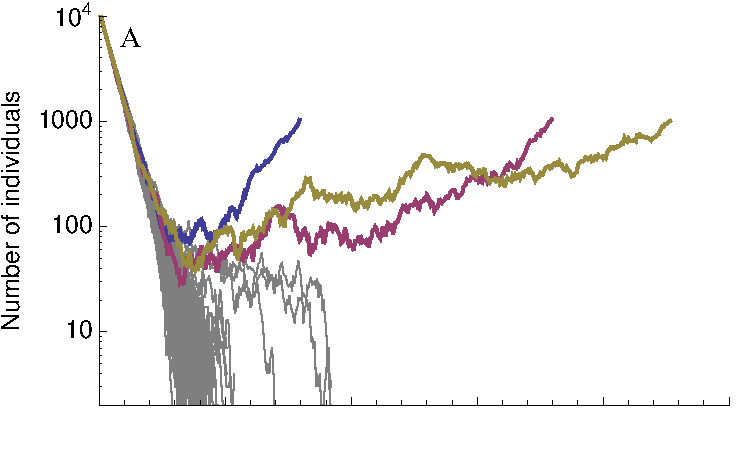
\includegraphics[width=\linewidth]{../IMAGES/Vshape.pdf}\\
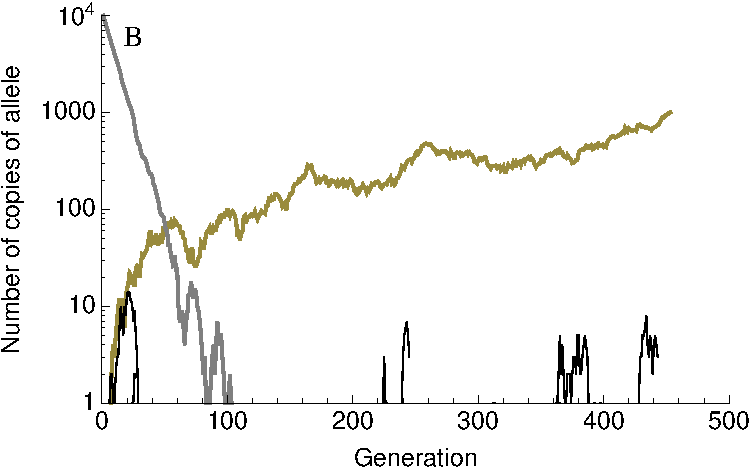
\includegraphics[width=\linewidth]{../IMAGES/VshapeMutations.pdf}
\caption{
Typical dynamics with a relatively slow wildtype decline and a small mutation rate ($m_0 = -0.1$, $U=10^{-4}$).
\textbf{(A)} Population size trajectories on a log scale.
Each line is a unique replicate simulation (100 replicates).
Replicates that went extinct are grey, replicates that were rescued are in colour (and are roughly V-shaped).
\textbf{(B)} The number of individuals with a given derived allele, again on a log scale, for the yellow replicate in \textbf{A}.
The number of individuals without any derived alleles (wildtypes) is shown in grey, the rescue mutation is shown in yellow, and all other mutations are shown in black.
Other parameters: $n=4$, $\lambda=0.005$, $m_{max}=0.5$.
}%
\label{fig:Vshape}
\end{figure}
%%%%%%%%%%%%%%%%%%%%%%%%%%%%%%%%%%%%%%%%%%%%%%%%%%%

As expected, V-shaped log-trajectories are the result of a single mutation creating a genotype with a positive growth rate that escapes loss when rare and rescues the population (Figure \ref{fig:Vshape}B), i.e., 1-step rescue.
U-shaped log-trajectories, on the other hand, occur when a single mutation creates a genotype with a negative (or potentially very small positive) growth rate, itself doomed to extinction, which out-persists the wildtype and gives rise to a double mutant genotype that rescues the population (Figure \ref{fig:Ushape}B), i.e., 2-step rescue. 
These two types of rescue comprise the overwhelming majority of rescue events observed in our simulations, across a wide range of wildtype decline rates (e.g., Figure \ref{fig:1vs2m0}).

Of course, with sufficiently high mutation rates rescue by 3 or more mutations comes to dominate (Figure \ref{fig:1vs2U}).
It has recently been suggested that when the mutation rate, $U$, is substantially less than a critical value, $U_C = \lambda n^2/4$, we are in a ``strong selection, weak mutation" regime where essentially all mutations arise on a wildtype background \citep{martin2016nonstationary}, consistent with the House of Cards approximation \citep{turelli1984heritable,turelli1985effects}, and thus rescue will occur by a single mutation of large effect \citep{Anciaux2018}.
In the other extreme, when $U>>U_C$, we are in a weak selection, strong mutation regime where many mutations arise on the same background, creating a multivariate normal phenotypic distribution \citep{martin2016nonstationary}, consistent with the Gaussian approximation \citep{Kimura1965,lande1980genetic}, and thus rescue will occur by many mutations of small effect \citep{anciaux2019population}.
As shown in Figure \ref{fig:1vs2m0} (where $U=U_C / 10$) and Figure \ref{fig:1vs2U} (which spans $U_C=0.02$), rescue by a small number of mutations (but more than one) can become commonplace in the transition zone, $U \sim U_C$, where there are often a considerable number of cosegregating mutations (e.g., Figure \ref{fig:Ushape}B, where $U = U_C/2$).

%%%%%%%%%%%%%%%%%%%%%%%%%%%%%%%%%%%%%%%%%%%%%%%%%%%
\begin{figure}[!h]
\centering
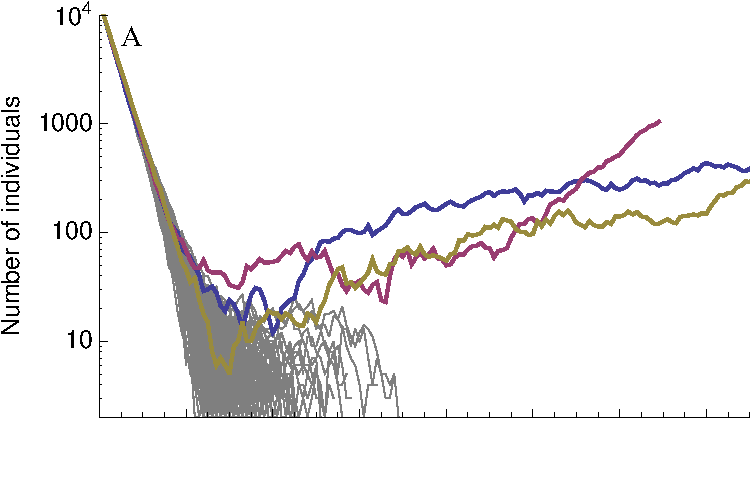
\includegraphics[width=\linewidth]{../IMAGES/Ushape.pdf}\\
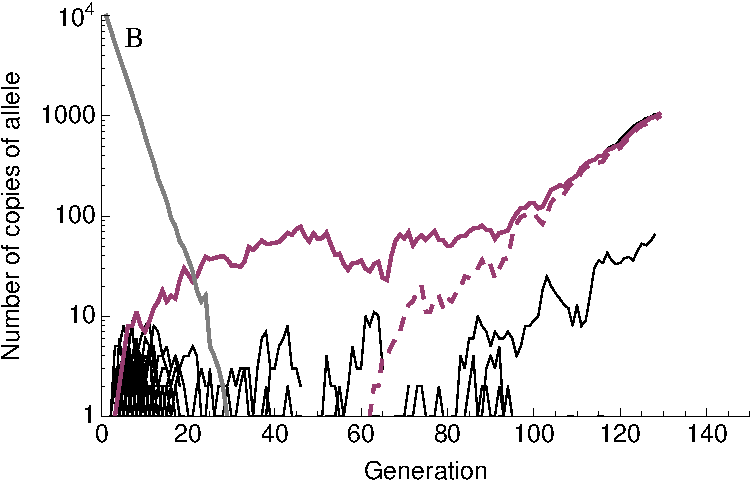
\includegraphics[width=\linewidth]{../IMAGES/UshapeMutations.pdf}
\caption{
Typical dynamics with a relatively fast wildtype decline and a large mutation rate ($m_0 = -0.3$, $U=10^{-2}$).
\textbf{(A)} Population size trajectories on a log scale.
Each line is a unique replicate simulation (500 replicates).
Replicates that went extinct are grey, replicates that were rescued are in colour.
Note that the blue and red replicates are cases of 2-step rescue (and roughly U-shaped), while the yellow replicate is 1-step rescue (and therefore V-shaped).
\textbf{(B)} The number of individuals with a given derived allele, again on a log scale, for the red replicate in \textbf{A}.
The number of individuals without any derived alleles (wildtypes) is shown in grey, the rescue mutations are shown in red, and all other mutations in black.
Here a single mutant with growth rate less than zero arises early and outlives the wildtype (solid red).
A second mutation then arises on that background (dashed red), making a double mutant with a growth rate greater than zero that rescues the population. 
Other parameters: $n=4$, $\lambda=0.005$, $m_{max}=0.5$.
}%
\label{fig:Ushape}
\end{figure}
%%%%%%%%%%%%%%%%%%%%%%%%%%%%%%%%%%%%%%%%%%%%%%%%%%%

\subsection{The probability of $k$-step rescue}

Approximations for the probability of 1-step rescue under the strong selection, weak mutation regime were derived by \cite{Anciaux2018}.  
Here we extend this study by exploring the contribution of $k$-step rescue, deriving approximations for the probability of such events, as well as dissecting the genetic basis of both 1- and 2-step rescue in terms of the distribution of fitness effects of rescue genotypes and their component mutations.

Although requiring a sufficiently beneficial mutations to arise on a rare mutant genotypes doomed to extinction, multi-step evolutionary rescue can be the dominant form of rescue when the wildtype is sufficiently maladapted (Figures \ref{fig:1vs2m0} and \ref{fig:1vs2U}). 
Indeed, on this fitness landscape, the probability of producing a rescue genotype in one mutational step mutant drops very sharply with maladaptation \citep{Anciaux2018}; mutants with intermediate growth rates can thus be a ``springboard" -- albeit not always a very bouncy one -- from which rescue mutants are produced. 
These intermediates contribute more as mutation rates and the decline rate of the wildtype increase (Figures \ref{fig:1vs2m0} and \ref{fig:1vs2U}); the former because double mutants become more likely and the latter because the springboard becomes more necessary.
With a large enough number of wildtype individuals or a high enough mutation rate (Figure \ref{fig:1vs2U}), multi-step rescue can not only be more likely than 1-step, but also very likely in an absolute sense.

\subsection{Alternative regimes of 2-step rescue}

2-step rescue can occur through first-step mutants with a wide range of growth rates. 
As shown below, these first-step mutants can be divided into three regimes: "sufficiently subcritical", "sufficiently critical", and "sufficiently supercritical" (we will often drop "sufficiently" for brevity; Figure \ref{fig:paths}).  
Critical first-step mutants are defined by having growth rates close enough to zero that occasionally such a mutation will, by chance, persist for long enough that it will almost certainly produce successful double mutants.
Subcritical first-step mutants are then defined by having growth rates that are negative enough to prevent such long persistence times. 
Their dynamics are roughly deterministic; mutations conferring growth rates closer to zero persist longer but are less likely to arise from the wildtype.
Similarly, supercritical first-step mutants are defined by having positive growth rates that are large enough to prevent long persistence times once conditioned on extinction; conditioned on extinction these genotypes behave like subcritical mutations with a growth rate of the same absolute value \citep{maruyama1974note}.
As with subcritical first-step mutants, the dynamics of supercritical mutants are relatively deterministic, but in this case persistence times and mutational input from the wildtype both favour growth rates closer to zero.

The relative contribution of each regime changes with both the initial degree of maladaptation and the mutation rate (Figures \ref{fig:2stepstyle} and \ref{fig:firststepDFE_mutation}).
When the wildtype is very maladapted (relative to mutational variance), most 2-step rescue events occur through subcritical first-step mutants (Figure \ref{fig:2stepstyle}A), which are more abundant than critical or supercritical mutants and yet persist longer than the wildtype.
If the initial maladaptation is milder, however, the slow decline of the wildtype buys time for critical and supercritical mutations to arise and contribute to 2-step rescue, and also increases the rate at which they are produced. 
The rate of mutation also plays an interesting role in determining the relative contributions of each regime (Figures \ref{fig:2stepstyle}B and \ref{fig:firststepDFE_mutation}). 
When mutations are rare, only first-step mutations that are very nearly neutral ($m\sim0$) will persist long enough to give rise to a 2-step rescue mutation. 
As the mutation rate increases, however, the range of first-step mutant growth rates that can persist long enough to lead to 2-step rescue widens (because fewer individuals carrying the first-step mutation are needed to produce a successful double mutant).

\subsection{The distribution of fitness effects among rescue mutations}

Mutants causing 1-step rescue have growth rates that cluster around small positive values ($m\gtrsim 0$; Figure \ref{fig:1and2stepDFE}).
Consequently, the distribution of fitness effects (DFE) is shifted to the right relative to the constant population size case, beginning at $s= m - m_0 \geq -m_0 > 0$.
As a result of this increased threshold, the 1-step rescue DFE has a smaller variance than both the DFE of random mutations and the DFE of mutations that establish in a constant population \citep{Kimura1983}. 
Further, unlike these other distributions, the variance in the DFE under 1-step rescue decreases as the rate of wildtype decline increases, due to rescue being restricted to a smaller proportion of the available mutants.

The DFE of genotypes that cause 2-step rescue (the combined effect of two mutations) is also clustered at small positive values, but it has a variance that is less affected by the rate of wildtype decline (Figure \ref{fig:1and2stepDFE}).
This is because double mutant rescue genotypes are created via first-step mutant genotypes that have larger growth rates than the wildtype (i.e., are closer to the optimum), allowing them to create double mutants with a larger range of positive growth rates.

Finally, we can also look at the distribution of growth rates among firsts-step mutations that lead to 2-step rescue (Figures \ref{fig:2stepDFE} and \ref{fig:firststepDFE_mutation}), i.e., 'springboard mutants'.
Here there are two main factors to consider: 1) the probability that a mutation with a given growth rate arises on the wildtype background but does not by itself rescue the population and 2) the probability that such a mutation persists long enough for a sufficiently beneficial second mutation to arise on that same background and together rescue the population. 
As explained above, increasing the rate of wildtype decline (or decreasing the rate of mutation) shifts the contribution from critical first-step mutants to subcritical first-step mutants, lowering the mode and increasing the variance.

Finally, note that, given 2-step rescue, the growth rate of both the first and second mutation may be negative when alone in the wildtype background. 
This potentially obscures empirical detection of the individual mutations involved in evolutionary rescue. 

%%%%%%%%%%%%%%%%%%%%%%%%%%%%%%%%%%%%%%%%%%%%%%%%%%%
%%%%%%%%%%%%%%%%%%%%%%%%%%%%%%%%%%%%%%%%%%%%%%%%%%%
\section{Mathematical Analysis}
\label{sec:analysis}

\begin{table}[!h]
\begin{tabular}{p{1.5cm} p{6.5cm}}
\hline
Symbol & Meaning \\
\hline
\hline
$n$ & number of (scaled) phenotypic dimensions\\
$\lambda$ & variance in mutant phenotypes along each dimension\\
%$\vec{z}$ & $n$ dimensional trait vector\\
%$\vec{o}$ & optimal trait value\\
%$m(\vec{z}) = \ln W(\vec{z})$ & Malthusian growth rate of phenotype $\vec{z}$\\
$m_{max}$ & maximum growth rate\\
%$s = m'-m$ & fitness effect of mutant with growth rate $m'$ relative to wildtype with growth rate $m$\\
%$s_o=m_{max}-m$ $ fitness effect of optimal phenotype relative to wildtype with growth rate $m$\\ 
$f(m'|m)$ & distribution of growth rates among mutants from a genotype with growth rate $m$ (eq.\ \ref{eq:fm})\\
$U$ & per genome mutation probability\\ 
$N_0$ & initial number of wildtype individuals\\
%$\vec{z}_0$ & wildtype phenotype\\
$m_0$ & wildtype growth rate\\
$p_0$ & probability that an initial wildtype individual has descendants that rescue the population\\
$P$ & probability of rescue (eq.\ \ref{eq:Prescue})\\
%$U_C = \frac{\lambda n^2}{4}$ & proposed threshold between mutational regimes\\
$p(m,\Lambda(m))$ & probability a genotype with growth rate $m$, itself fated for extinction, has descendants that rescue the population (eq.\ \ref{eq:S15})\\
$p_{est}(m)$ & probability a genotype with growth rate $m$ establishes, i.e., rescues the population (eq.\ \ref{eq:pestm})\\
$\Lambda(m)$ & probability that an individual with growth rate $m$ produces a mutant that has descendants that rescue the population\\
$\Lambda_i(m)$ & probability that an individual with growth rate $m$ produces a mutant that has descendants with $i-1$ additional mutations that rescue the population\\
%$\tilde{\Lambda}_1(m)$ & closed-form approximation of $\Lambda_1(m)$ (eq.\ \ref{eq:p1closed})\\
%$m^*$, $-m^*$ & approximate cutoffs between sufficiently critical and non-critical first-step mutants\\
%$\Lambda_2^{(-)}(m)$ & rate at which a genotype with growth rate $m$ produces sufficiently subcritical first-step mutants that lead to 2-step rescue (Equation \ref{eq:p2tilde}) \\
%$\Lambda_2^{(0)}(m)$ & rate at which a genotype with growth rate $m$ produces sufficiently critical first-step mutants that lead to 2-step rescue (Equation \ref{eq:p2tilde})\\
%$\Lambda_2^{(+)}(m)$ & rate at which a genotype with growth rate $m$ produces sufficiently supercritical first-step mutants that lead to 2-step rescue (Equation \ref{eq:p2tilde})\\
$\Lambda_2^{(-)}(m)$, $\Lambda_2^{(0)}(m)$, $\Lambda_2^{(+)}(m)$ & probability that an individual with growth rate $m$ produces sufficiently subcritical, critical, or supercritical first-step mutants that eventually lead to 2-step rescue (eq.\ \ref{eq:p2tilde}) \\
%$\tilde{m}^*$ & \\
$\psi$ & $2(1-\sqrt{1-m/m_{max}})$ \\
$\psi_0$ & $2(1-\sqrt{1-m_0/m_{max}})$\\
%$\psi_-^*$\\
%$\psi_+^*$\\
%$\psi_{max}$\\
$\rho_{max}$ & $m_{max}/\lambda$\\
$\alpha$ & $\rho_{max} \psi_0^2/4$\\
%$g_1(m)$ & distribution of growth rates among 1-step rescue genotypes (eq.\ \ref{eq:g1m})\\
%$\tilde{g}_1(\psi)$ & scaled, closed-form approximation of $g_1(m)$ (eq.\ \ref{eq:tildeg1m})\\
%$g_2(m)$ & distribution of growth rates among 2-step rescue genotypes (eq.\ \ref{eq:g2m})\\
%$h(m)$ & distribution of growth rates among first-step mutants that lead to 2-step rescue (eq.\ \ref{eq:hm})\\
\hline
\end{tabular}
\caption{Frequently used notation.}
\label{tab:notation}   
\end{table}

\subsection{The probability of $k$-step rescue}

Generic expressions for the probability of 1- and 2-step rescue were given by \cite{Martin2013}, using a diffusion approximation of the underlying demographics.
The key result that we will use is the probability that a single copy of a genotype with growth rate $m$, itself fated for extinction but which produces rescue mutants at rate $\Lambda(m)$, rescues the population \citep[equation S1.5 in][]{Martin2013}.
With our lifecycle this is \citep[c.f., equation A.3 in][]{Iwasa2004}

\begin{equation}\label{eq:S15}
\begin{aligned}
p(m,\Lambda(m)) 
   &= 1 - \exp \left[  |m| \left(1 - \sqrt{1+\frac{2\Lambda(m)}{m^2}} \right) \right].
\end{aligned}
\end{equation}

\noindent We can therefore use $p_0 = p(m_0,\Lambda(m_0))$ as the probability that a wildtype individual has descendants that rescue the population and what remains in calculating the total probability of rescue (Equation \ref{eq:Prescue}) is $\Lambda(m_0)$.
We break this down by letting $\Lambda_i(m)$ be the rate at which rescue genotypes with $i$ mutations are created; the total probability of rescue is then given by Equation \ref{eq:Prescue} with $p_0=p(m_0, \sum_{i=1}^\infty\Lambda_i(m_0))$.

In 1-step rescue, $\Lambda_1(m_0)$ is just the rate of production of rescue mutants directly from a wildtype genotype.
This is the probability that a wildtype gives rise to a mutant with growth rate $m$ (given by $U f(m|m_0)$) times the probability that a genotype with growth rate $m$ establishes.
Again approximating our discrete time process with a diffusion process, the probability that a lineage with growth rate $m<<1$ establishes, ignoring further mutation, is \citep{Martin2013}

\begin{equation}\label{eq:pestm}
p_{est}(m) \approx
\begin{cases}
	0 & m \leq 0 \\
	1-\exp(-2 m) & m > 0
\end{cases}.
\end{equation}

\noindent This reduces to the $2(s+m_{0})$ result in \cite{Otto1997} when $m = s + m_{0}$ is small, which further reduces to $2s$ in a population of constant size, $m_{0}=0$ \citep{Haldane1927}.
Using this, the rate of 1-step rescue is

\begin{equation}\label{eq:Lambda1}
\Lambda_1(m_0) = U \int_0^{m_{max}} f(m|m_0) p_{est}(m) \mathrm{d}m.
\end{equation}

\noindent Taking the first order approximation of $p(m_0,\Lambda_1(m_0))$ with $\Lambda_1(m_0)/m_0^2$ small gives the probability of 1-step rescue given in equation 5 of \cite{Anciaux2018}, which effectively assumes deterministic wildtype decline.
For completeness we rederive their closed-form approximation in File S1 (and give the results in the Appendix, see \nameref{subsec:1stepApproximations}).

The probability of 2-step rescue is only slightly more complicated.
Here $\Lambda_2(m_0)$ is the probability that a mutation arising on the wildtype background creates a genotype that is also fated for extinction but persists long enough for a second mutation to arise on this mutant background, creating a double mutant genotype that rescues the population.
We therefore have

\begin{equation}\label{eq:Lambda2}
\begin{aligned}
\Lambda_2(m_0) = U \int_{-\infty}^{m_{max}} f(m|m_0) \left[ 1 - p_{est}(m) \right] p(m,\Lambda_{1}(m)) \mathrm{d}m.
\end{aligned}
\end{equation}

Following this logic, we can retrieve the probability of $k$-step rescue, for arbitrary $k\geq2$,  using the recursion

\begin{equation}\label{eq:Lambdak}
\begin{aligned}
\Lambda_k(m_0) =& U \int_{-\infty}^{m_{max}} f(m|m_0) \left[ 1 - p_{est}(m) \right] \\
                       & p(m,\Lambda_{k-1}(m)) \mathrm{d}m,
\end{aligned}
\end{equation}

\noindent with the initial condition given by Equation \ref{eq:Lambda1}.

%%%%%%%%%%%%%%%%%%%%%%%%%%%%%%%%%%%%%%%%%%%%%%%%%%%
\begin{figure}[htb]
\centering
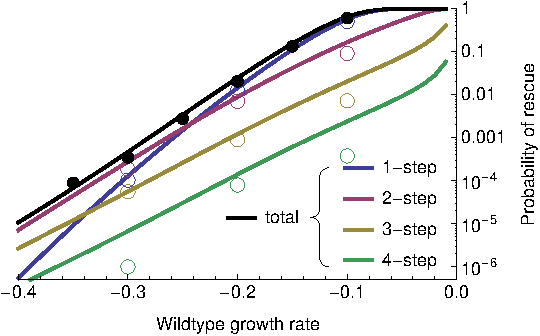
\includegraphics[width=\linewidth]{../IMAGES/4stepNormalU_sims.pdf}
\caption{
The probability of evolutionary rescue as a function of initial maladaptation.
Shown are the probabilities of 1-, 2-, 3-, and 4-step rescue (Equations \ref{eq:Prescue}-\ref{eq:Lambdak}), as well as the probability of rescue by up to 4 mutational steps (using $\Lambda(m_0) = \sum_{i=1}^4 \Lambda_i(m_0)$).
Dots are individual-based simulation results (ranging from $10^3$ to $10^5$ replicates per dot), allowing any number of mutations.
Simulated populations were considered rescued when there were 1000 individuals with positive growth rates.
Parameters: $N_0=10^4$, $U=2\times10^{-3}$, $n=4$, $\lambda=0.005$, $m_{max}=0.5$.
}%
\label{fig:1vs2m0}
\end{figure}
%%%%%%%%%%%%%%%%%%%%%%%%%%%%%%%%%%%%%%%%%%%%%%%%%%%

\subsection{Approximating the probability of 2-step rescue}

The probability of 2-step rescue is given by Equation \ref{eq:Prescue} with $p_0=p(m_0,\Lambda_2(m_0))$ (Equations \ref{eq:S15}-\ref{eq:Lambda2}).
We next develop some intuition by approximating this for different classes of single mutants.

First, note that when the growth rate of a first-step mutation is close enough to zero such that $m^2 << \Lambda_1(m)$, we can approximate the probability such a genotype leads to rescue before itself going extinct, $p(m,\Lambda_1(m))$, with $\sqrt{2\Lambda_1(m)}$ \citep[c.f.\ equation A.4b in ][]{Iwasa2004}.
As shown in the Appendix (see \nameref{subsec:mutants}), while $t<1/|m|$ a mutant lineage with growth rate $m$ that is destined for extinction persists for $t$ generations with probability $\sim2/t$ (Equation \ref{eq:pT}) and in generation $t$ since it has arisen has $\sim t/2$ individuals (Equation \ref{eq:pnt}). 
Thus, while $T<1/|m|$ a mutant lineage that persists for $T$ generations will have produced a cumulative number $\sim T^2/4$ individuals. 
Such lineages will then lead to 2-step rescue with probability $\sim \Lambda_1(m) T^2/4$ until this approaches 1, near $T=2/\sqrt{\Lambda_1(m)}$.
Since the probability of rescue increases like $T^2$ while the probability of persisting to time $T$ declines only like $1/T$, most rescue events will be the result of rare long-lived single mutant genotypes.
Considering only the most long-lived genotypes, the probability a first-step mutation leads to rescue is then the probability it survives long enough to almost surely rescue, $\sim2/\sqrt{\Lambda_1(m)}$ generations.
Thus, for first-step mutants with growth rates satisfying $2/\sqrt{\Lambda_1(m)} < 1/|m|$, implying $m^2 << \Lambda_1(m)$, such that they can by chance persist for unusually long times, the probability they lead to rescue is $\sim\sqrt{\Lambda_1(m)}$, consistent with our Taylor series approximation of $p(m,\Lambda_1(m))$.
This same reasoning has been used to explain why the probability a neutral mutation segregates long enough to produce a second mutation is $\sim\sqrt{U}$ in a population of constant size \citep{Weissman2009}.

At the other extreme, when the growth rate of a first-step mutation is far enough from zero such that $m^2 >> \Lambda_1(m)$, we can approximate $p(m,\Lambda_1(m))$ with $\Lambda_1(m)/ |m|$ \citep[c.f.\ equation A.4c in ][]{Iwasa2004}.
As just discussed, conditioned on extinction such genotypes cannot persist long enough to almost surely lead to 2-step rescue.
Instead, we expect such mutations to persist for at most $\sim1/|m|$ generations (Equation \ref{eq:pT}) with a lineage size of $\sim1$ individual per generation (Equation \ref{eq:pnt}), and thus produce a cumulative total of $\sim 1/|m|$ individuals. 
The probability of 2-step rescue from such a first-step mutation is therefore $\Lambda_1(m)/ |m|$, again consistent with our Taylor series approach.
This is the same reasoning that explains why a rare mutant genotype with selection coefficient $|s|>>0$ in a constant population size model is expected to have a cumulative number $\sim1/|s|$ individuals, given it eventually goes extinct \citep{Weissman2009}. 

The transitions between these two regimes occur when $\Lambda_1(m)/ |m| = \sqrt{2\Lambda_1(m)}$, i.e., when $|m| = \sqrt{\Lambda_1(m)/2}$.
We call single mutants with growth rates $m < -\sqrt{\Lambda_1(m)/2}$ "sufficiently subcritical", those with $|m| < \sqrt{\Lambda_1(m)/2}$ "sufficiently critical", and those with $m > \sqrt{\Lambda_1(m)/2}$ "sufficiently supercritical".
Given that $U$ and thus $\Lambda_1(m)$ will generally be small, $m$ will also be small at these transition points, meaning we can approximate them with $m^* = \sqrt{\Lambda_1(0)/2}$ and $-m^*$.
We then have an approximation for the rate of 2-step rescue, 

\begin{equation}\label{eq:p2tilde}
\begin{aligned}
&\Lambda_2(m_0) = \Lambda_2^{(-)}(m_0) + \Lambda_2^{(0)}(m_0) + \Lambda_2^{(+)}(m_0)\\
& \Lambda_2^{(-)}(m_0) = U \int_{-\infty}^{-m^*} f(m|m_0)  \Lambda_1(m)/ |m| \mathrm{d}m\\
& \Lambda_2^{(0)}(m_0) = U \int_{-m^*}^{m^*} f(m|m_0) \left[ 1 - p_{est}(m) \right] \sqrt{2\Lambda_1(m)} \mathrm{d}m\\
& \Lambda_2^{(+)}(m_0) = U \int_{m^*}^{m_{max}} f(m|m_0) \left[ 1 - p_{est}(m) \right] \Lambda_1(m)/ |m| \mathrm{d}m
\end{aligned}
\end{equation}

\noindent where $\Lambda_2^{(-)}(m_0)$ is the rate of 2-step rescue through sufficiently subcritical first-step mutants, $\Lambda_2^{(0)}(m_0)$ is the rate of 2-step rescue through sufficiently critical first-step mutants, and $\Lambda_2^{(+)}(m_0)$ is the rate of 2-step rescue through sufficiently supercritical first-step mutants.
A schematic depicting the 1- and 2-step genetic paths to rescue is given in Figure \ref{fig:paths}.

%%%%%%%%%%%%%%%%%%%%%%%%%%%%%%%%%%%%%%%%%%%%%%
\begin{figure}[htb]
\centering
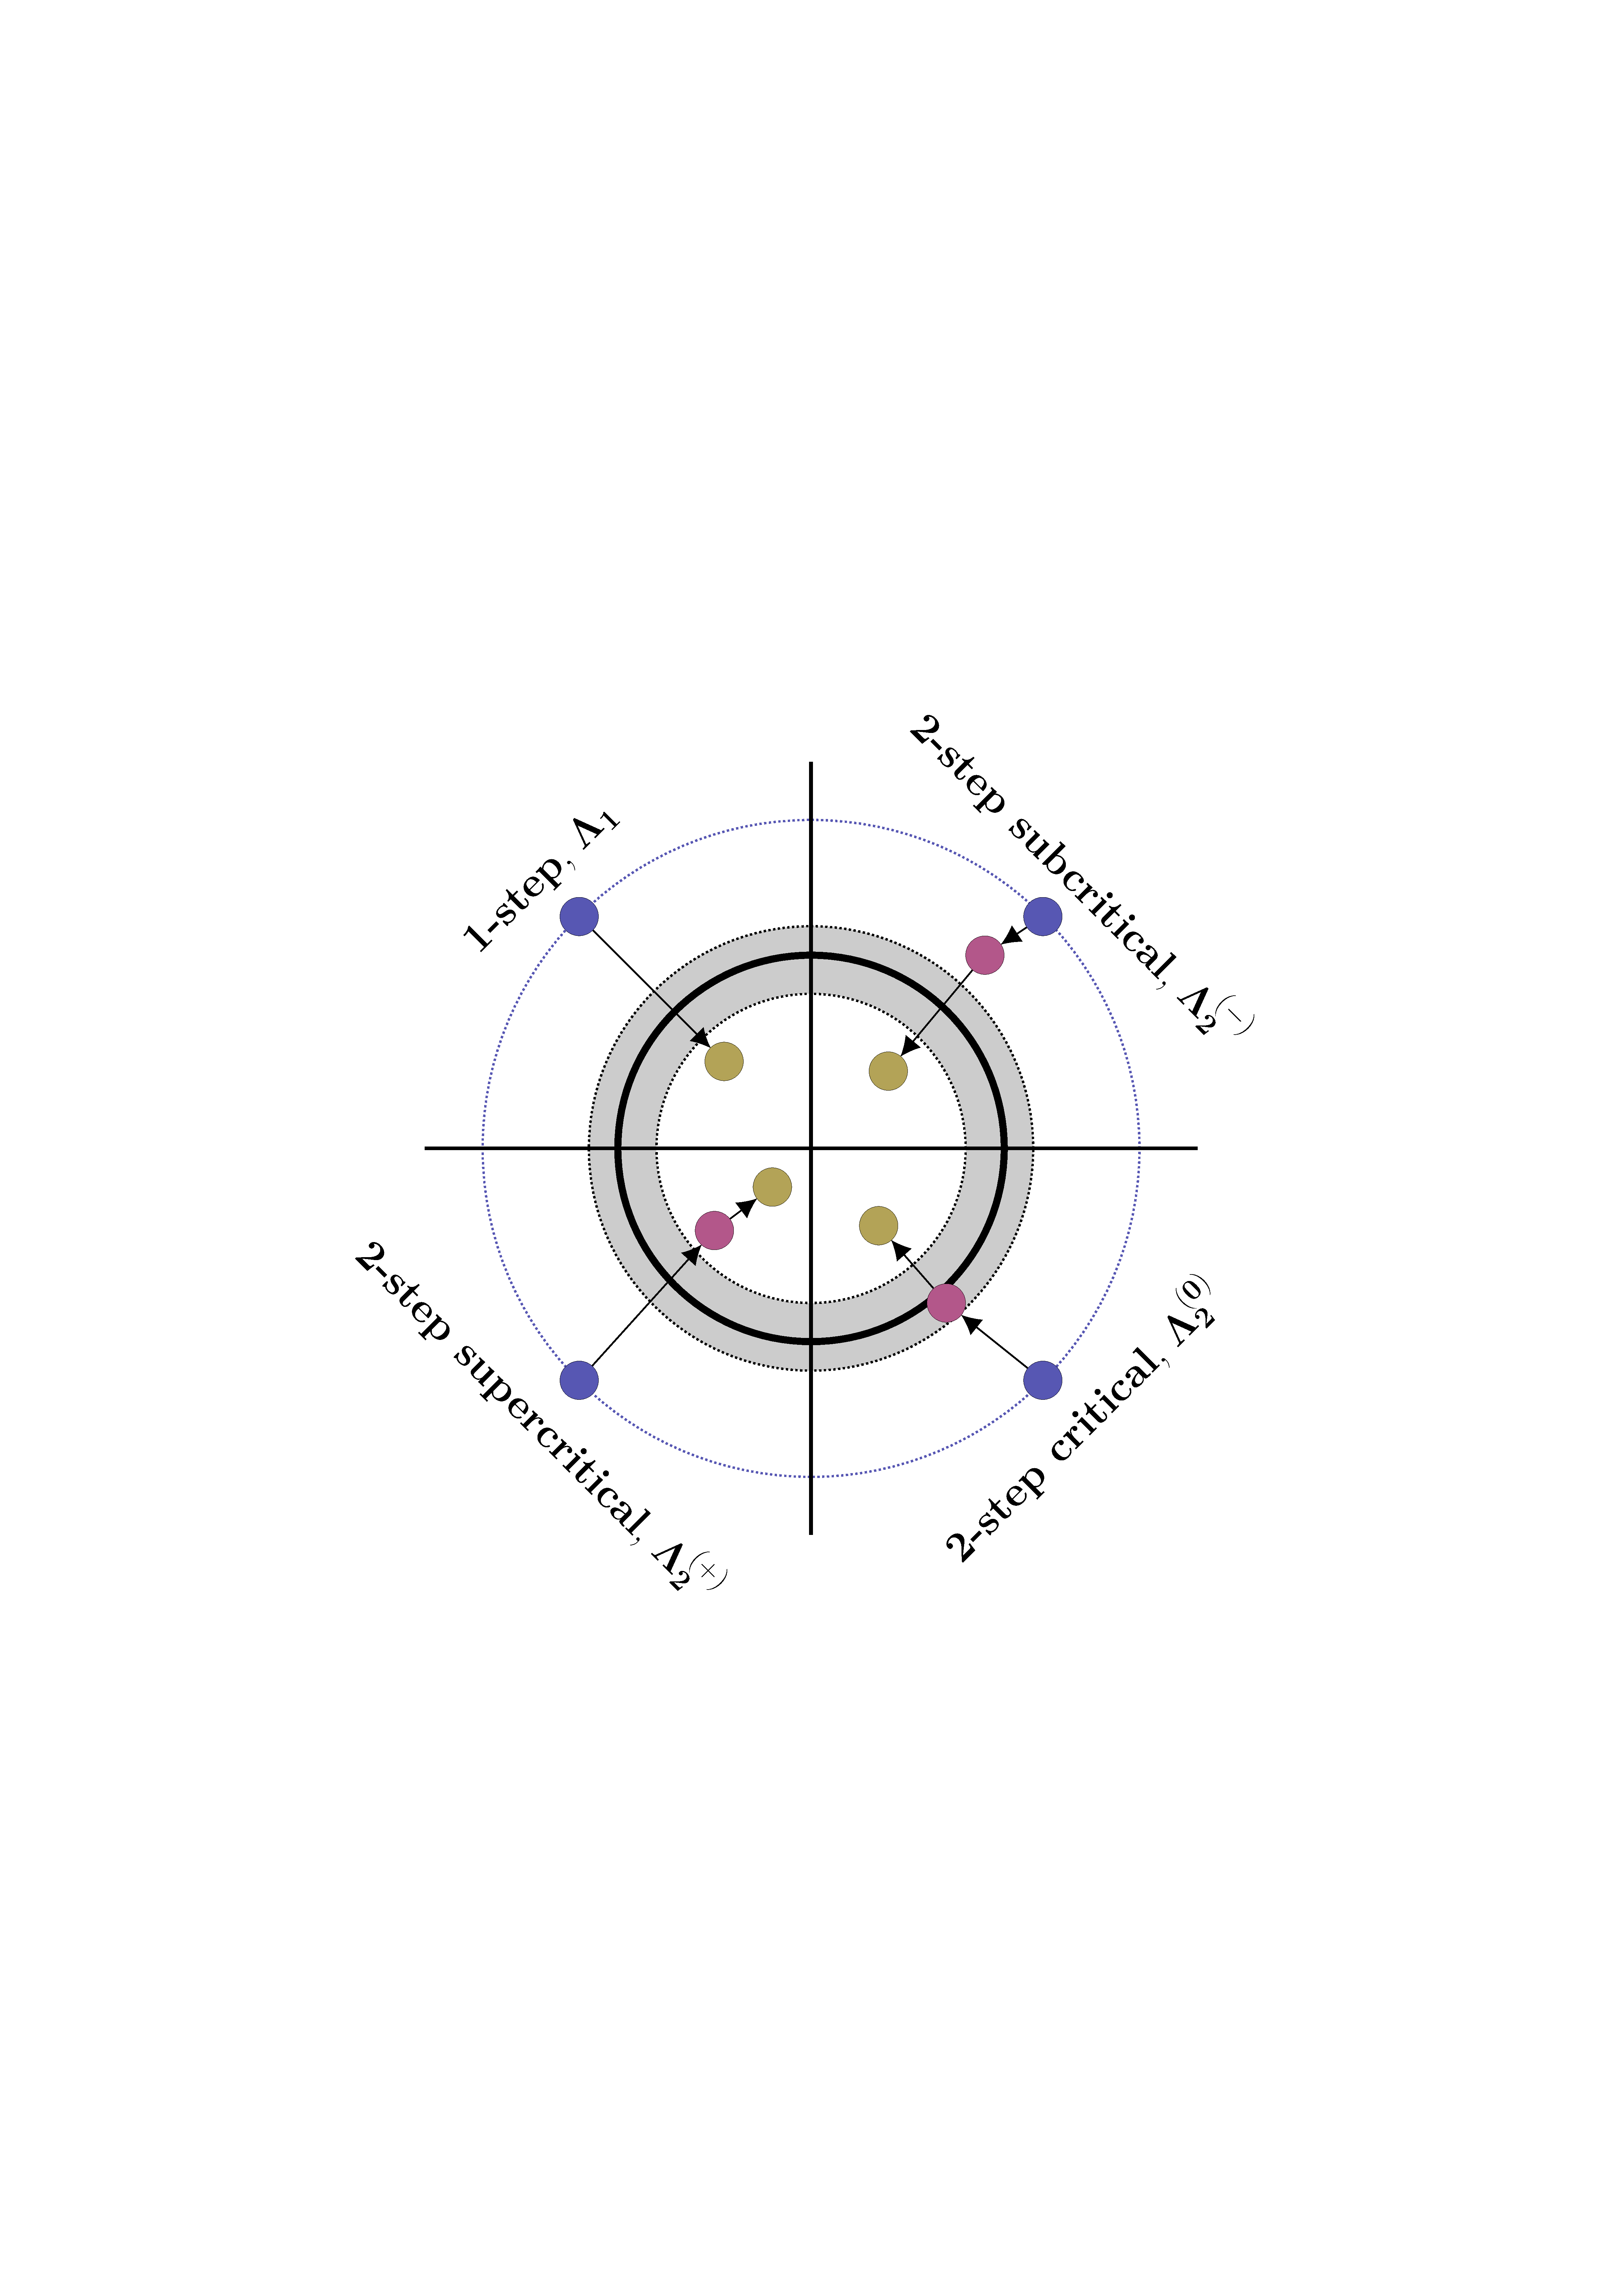
\includegraphics[width=\linewidth, trim = {14cm, 35cm, 14cm, 35cm}, clip]{../IMAGES/fgmer_diagrams_code.pdf}
\caption{
1- and 2-step genetic paths to evolutionary rescue.
Here we show an $n=2$ dimensional phenotypic landscape.
Continuous-time (Malthusian) growth rate ($m$) declines quadratically from the centre, becoming negative outside the thick black line.
The grey zone indicates where growth rates are ``sufficiently critical" (see text for details).
Blue circles show wildtype phenotypes, red circles show intermediate first-step mutations, and yellow circles show the phenotypes of rescue genotypes.
}%
\label{fig:paths}
\end{figure}
%%%%%%%%%%%%%%%%%%%%%%%%%%%%%%%%%%%%%%%%%%%%%%

\subsubsection{Closed-form approximation for sufficiently critical rescue}

When $U$ is small $m^*$ is also small, allowing us to use $m = 0$ within the integrand of $\Lambda_2^{(0)}(m_0)$, giving 

\begin{equation}\label{eq:p20app1}
\begin{aligned}
\Lambda_2^{(0)}(m_0)
&\approx U f(0|m_0)  \sqrt{2\Lambda_1(0)} 2m^*\\
&= 2 U f(0|m_0) \Lambda_1(0).
\end{aligned}
\end{equation}

\noindent We can then approximate $\Lambda_1(m)$ with $\tilde{\Lambda}_1(m)$ (Equation \ref{eq:p1closed}) and take $m\rightarrow0$ (Equation \ref{eq:Lambda0}), giving a closed form approximation for the rate of 2-step rescue through critical single mutants in Fisher's geometric model

\begin{equation}\label{eq:p20app}
\begin{aligned}
\Lambda_2^{(0)}(m_0)
&\approx 4 U^2 f(0|m_0)  \sqrt{m_{max} \lambda/ \pi}.
\end{aligned}
\end{equation}

\noindent This well approximates numerical integration of $\Lambda_2^{(0)}(m_0)$  (Equation \ref{eq:p2tilde}; see Figure \ref{fig:2stepstyle} and File S1) .
In general, it will perform better as the range of critical growth rates, and thus $U \sqrt{m_{max} \lambda}$, becomes smaller.

To get a better understanding of how the rate of 2-step critical rescue depends on the underlying parameters of Fisher's geometric model, we approximate $f(m|m_0)$, assuming $\rho_{max} = m_{max}/\lambda$ is large, and convert this to a distribution over $\psi = 2(1-\sqrt{1-m/m_{max}})$, a convenient rescaling \citep[for details seeFile S1 and][]{Anciaux2018}.
Evaluating this at $m=0$ gives

\begin{equation}\label{eq:p20app2}
\begin{aligned}
\Lambda_2^{(0)}(m_0)
&\approx U^2 (1-\psi_0/2)^{(1-n)/2} e^{-\alpha} \frac{2}{\pi},
\end{aligned}
\end{equation}

\noindent where $\psi_0 = 2(1-\sqrt{1-m_0/m_{max}})$ and $\alpha = \rho_{max} \psi_0^2/4$.

\subsubsection{Closed-form approximations for sufficiently non-critical rescue}

We can also approximate $\Lambda_1(m)$ in $\Lambda_2^{(-)}(m_0)$ and $\Lambda_2^{(+)}(m_0)$ with $\tilde{\Lambda}_1(m)$ (Equation \ref{eq:p1closed}), leaving us with just one integral over the growth rates of the first-step mutations.
We then replace $f(m|m_0)$ with its approximate distribution over $\psi$.

In the case of subcritical rescue we can then make two contrasting approximations.
First, when the $\psi$ (and thus $m$) that contribute most are close enough to zero (meaning maladaptation is not too large relative to mutational variance) and we ignore mutations that are less fit than the wildtype, we have

\begin{equation}\label{eq:Lambda2_smallPsi}
\Lambda_2^{(-)}(m_0) \approx U^2 \frac{(1-\psi_0/2)^{1-n}}{1-\psi_0/4} e^{-\alpha} \frac{\log(\psi_0 / \psi^*_{-})}{\pi},
\end{equation}

\noindent where $\psi^*_{-} = 2(1-\sqrt{1 + \tilde{m}^*/m_{max}})$ and $\tilde{m}^* = \sqrt{\tilde{\Lambda}_1(0)/2}$.
Second, when the mutational variance, $\lambda$, is very small relative to maladaptation, implying that mutants far from $m=0$ substantially contribute, we find

\begin{equation}\label{eq:Lambda2_largeRho}
\Lambda_2^{(-)}(m_0) \approx -U^2 \frac{(1-\psi_0/2)^{1-n}}{1-\psi_0/4} \left(  e^{-\alpha} \frac{1}{(\alpha/2)^3 \pi} \right)^{1/2}.
\end{equation}

\noindent These two approximations do well compared with $\Lambda_2^{(-)}(m_0)$ (Equation \ref{eq:p2tilde}; see Figure \ref{fig:2stepstyle} and File S1).
As expected, we find that Equation \ref{eq:Lambda2_largeRho} does better under fast wildtype decline while Equation \ref{eq:Lambda2_smallPsi} does better when the wildtype is declining more slowly. 

For supercritical 2-step rescue, only first-step mutants with growth rates near $m^*$ will contribute (larger $m$ will rescue themselves and are also less likely to arise by mutation), and so we can capture the entire distribution with a small $m$ approximation (following the same approach that led to Equation \ref{eq:Lambda2_smallPsi}).
As shown in File S1, this approximation works well for $\psi<\sqrt{2/\rho_{max}}$, beyond which the rate of 2-step rescue through such first-step mutants falls off very quickly due to a lack of mutational input.
Thus, considering only supercritical single mutants with scaled growth rate less than $\sqrt{2/\rho_{max}}$, our approximation is

\begin{equation}\label{eq:Lambda2_smallPsi_Super}
\Lambda_2^{(+)}(m_0) \approx U^2 \frac{(1-\psi_0/2)^{1-n}}{1-\psi_0/4} e^{-\alpha} \frac{\log(\psi_{max} / \psi^*_{+})}{\pi},
\end{equation}

\noindent with $\psi^*_{+} = 2(1-\sqrt{1 - \tilde{m}^*/m_{max}})$ and $\psi_{max} = \sqrt{2/\rho_{max}}$.
This approximation tends to provide a slight overestimate of $\Lambda_2^{(+)}(m_0)$ (Equation \ref{eq:p2tilde}; see Figure \ref{fig:2stepstyle} and File S1).

\subsubsection{Comparing 2-step regimes}

These rough but simple closed-form approximations (Equations \ref{eq:p20app2}--\ref{eq:Lambda2_smallPsi_Super}) show that, while the contribution of critical mutants to 2-step rescue scales with $U^2$, the contribution of non-critical single mutants scales at a rate less than $U^2$ due to an increase in the range of critical single mutants (both $\psi^*_-$ and $\psi^*_+$ increase with $U$).
This difference in scaling with $U$ is stronger when the wildtype is not very maladapted relative to the mutational variance, i.e., when Equation \ref{eq:Lambda2_smallPsi} is the better approximation for subcritical rescue.
The approximations also show that, when initial maladaptation is small the ratio of supercritical to subcritical contributions (Equation \ref{eq:Lambda2_smallPsi} divided by \ref{eq:Lambda2_smallPsi_Super}) primarily depends only on the range of growth rates included in each regime, while with larger initial maladaptation this ratio (Equation \ref{eq:Lambda2_largeRho} divided by \ref{eq:Lambda2_smallPsi_Super}) begins to depend more strongly on initial maladaptation and mutational variance ($\alpha$).
The effect of maladaptation and mutation rate on the relative contributions of each regime is shown in Figure \ref{fig:2stepstyle}.

%%%%%%%%%%%%%%%%%%%%%%%%%%%%%%%%%%%%%%%%%%%%%%
\begin{figure}[htb]
\centering
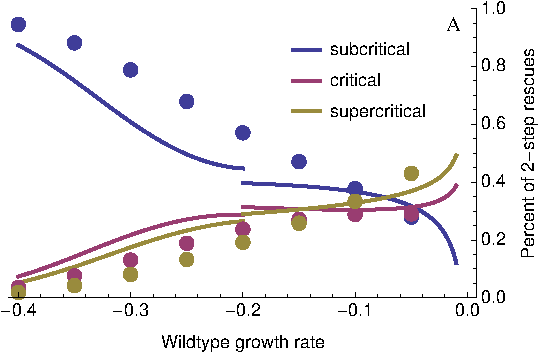
\includegraphics[width=\linewidth]{../IMAGES/p2RelContrGrowth.pdf}\\
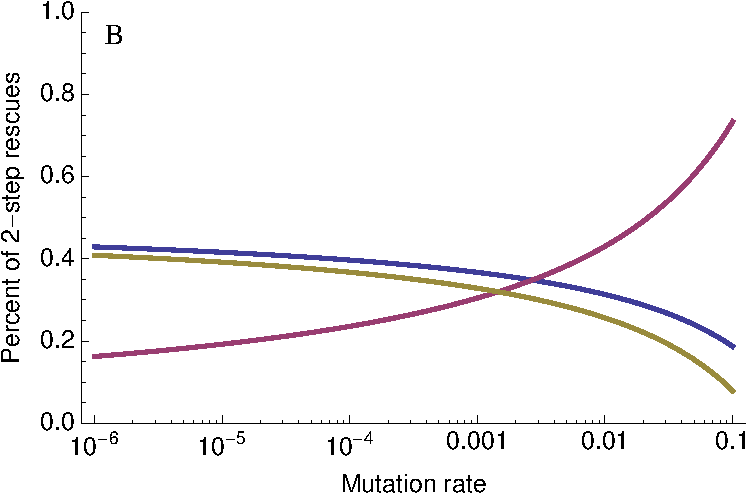
\includegraphics[width=\linewidth]{../IMAGES/p2RelContrMutationSlow.pdf}
\caption{
The relative contribution of sufficiently subcritical, sufficiently critical, and sufficiently supercritical single mutants to 2-step rescue.
The curves are drawn using Equations \ref{eq:p20app}--\ref{eq:Lambda2_smallPsi_Super} (Equation \ref{eq:Lambda2_smallPsi} is used for $m_0<0.2$ while Equation \ref{eq:Lambda2_largeRho} is used for $m_0>0.2$).
The dots are numerical evaluations of Equation \ref{eq:p2tilde}.
Parameters: $n=4$, $\lambda=0.005$, $m_{max}=0.5$, (\textbf{A}) $U=10^{-3}$, (\textbf{B}) $m_0 = -0.1$.
}%
\label{fig:2stepstyle}
\end{figure}
%%%%%%%%%%%%%%%%%%%%%%%%%%%%%%%%%%%%%%%%%%%%%%

\subsection{The distribution of growth rates among rescue genotypes}

We next explore the distribution of growth rates among rescue genotypes, i.e., the distribution of growth rates that we expect to observe among the survivors across many replicates.

We begin with 1-step rescue.
The rate of 1-step rescue by genotypes with growth rate $m$ is simply $U f(m|m_0) p_{est}(m)$.
Dividing this by the rate of 1-step rescue through any $m$ (Equation \ref{eq:Lambda1}) gives the distribution of growth rates among the survivors

\begin{equation}\label{eq:g1m}
g_1(m) = \frac{U f(m|m_0) p_{est}(m)}{\Lambda_1(m_0)},
\end{equation}

\noindent where $U$ cancels out.
This distribution is shown in blue in Figure \ref{fig:1and2stepDFE}.
The distribution has a mode at small but positive $m$ as a result of two conflicting processes: smaller growth rates are more likely to arise from a declining wildtype but larger growth rates are more likely to establish given they arise. 
As the rate of wildtype decline increases, the former process exerts more influence, causing the mode to move towards zero and reducing the variance.

We can also give a closed form approximation here using the same approach taken to reach Equation \ref{eq:p1closed}.
On the $\psi$ scale we have

\begin{equation}\label{eq:tildeg1m}
\tilde{g}_1(\psi) = \frac{\exp(\alpha)\sqrt{\alpha \rho_{max}}}{[\exp(\alpha)\sqrt{\pi \alpha} \mathrm{Erfc}(\sqrt{\alpha}) - 1]\psi_0} e^{- \rho_{max} (\psi-\psi_0)^2/4} \psi,
\end{equation}

\noindent implying the $\psi$ are distributed like a normal truncated below $\psi=0$ and weighted by $\psi$.
This provides a very good approximation (see dashed blue curves in Figure \ref{fig:1and2stepDFE}).

In 2-step rescue, the rate of rescue by double mutants with growth rate $m_2$ is given by Equation \ref{eq:Lambda2} with $\Lambda_1(m)$ replaced by $U f(m_2|m) p_{est}(m_2)$.
Normalizing gives the distribution of growth rates among the double mutant genotypes that rescue the population

\begin{equation}\label{eq:g2m}
\begin{aligned}
&g_2(m_2) \approx \frac{A(m_2)}{\int_0^{m_{max}} A(m_2) \mathrm{d}m_2} \\
&A(m_2) = \int_{-\infty}^{m_{max}} f(m|m_0) \left[ 1 - p_{est}(m) \right] \\
&\hspace{2cm}p(m,U f(m_2|m) p_{est}(m_2))\mathrm{d}m.
\end{aligned}
\end{equation}

\noindent This distribution, $g_2(m)$, is shown in red in Figure \ref{fig:1and2stepDFE}.
Because the first-step mutants contributing to 2-step rescue tend to be nearer the optimum than the wildtype, this allows them to produce double mutant rescue genotypes with higher growth rates than in 1-step rescue (as seen by comparing the mode between blue and red curves in Figure \ref{fig:1and2stepDFE}).
The fact that these first-step mutants are closer to the optimum also allows for a greater variance in the growth rates of rescue genotypes than in 1-step rescue.
This also allows the 2-step distribution to maintain a more similar mode and variance across wildtype decline rate than the 1-step distribution. % as the wildtype growth rate varies.
Note that because the $U$ in $U f(m_2|m) p_{est}(m_2)$ does not cancel, $g_2(m_2)$ depends on $U$ and the buffering effect of first-step mutants depends on the mutation rate. 
In principle, decreasing the mutation rate disproportionately increases the contribution of first-step mutants with growth rates closer to zero, as these genotypes are more likely to persist long enough to produce rescue mutants (see \nameref{sec:m1DFE} below for more discussion).
This implies that the distribution of rescue genotype growth rates is more strongly buffered from the rate of wildtype decline at lower mutation rates.

%%%%%%%%%%%%%%%%%%%%%%%%%%%%%%%%%%%%%%%%%%%%%%%%%%%
\begin{figure}[htbp]
\centering
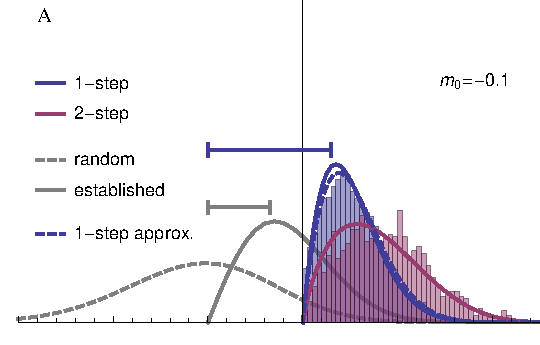
\includegraphics[width=\linewidth]{../IMAGES/2step_m2_smallm0_sims.pdf}\\
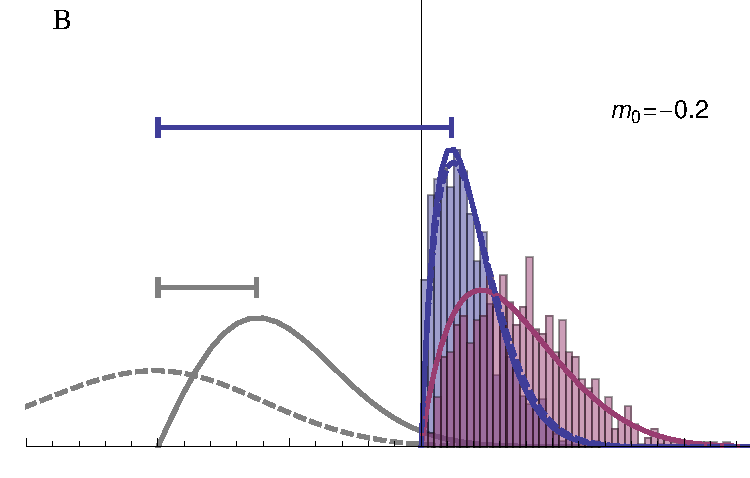
\includegraphics[width=\linewidth]{../IMAGES/2step_m2_medm0_sims.pdf}\\
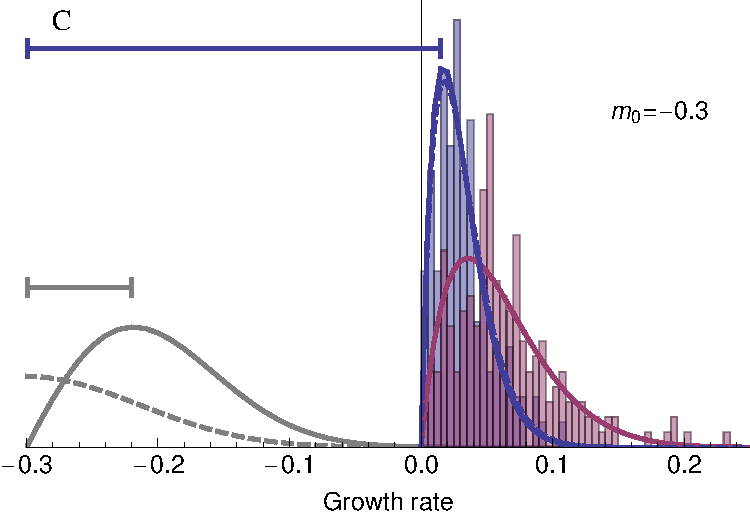
\includegraphics[width=\linewidth]{../IMAGES/2step_m2_largem0_sims.pdf}
\caption{
The distribution of growth rates among rescue genotypes under 1-step (blue; Equation \ref{eq:g1m} solid and \ref{eq:tildeg1m} dashed) and 2-step (red; Equation \ref{eq:g2m}) rescue for three different levels of initial maladaptation.
For comparison, the distribution of random mutations (dashed; Equation \ref{eq:fm}) and the distribution of beneficial mutations that establish in a population of constant size (solid grey; Equation \ref{eq:fm} times Equation \ref{eq:pestm} and normalized) are shown.
Horizontal lines indicate the most common fitness effect ($s=m_0-m$) in a population of constant size (grey) and in 1-step rescue (blue).
The histograms show the distribution of growth rates among rescue genotypes observed across (\textbf{A}) $10^4$, (\textbf{B}) $10^5$, and (\textbf{C}) $10^6$ simulated replicates.
Populations were considered rescued once there were $\geq$100 individuals with positive growth rate.
The most common genotype at this point was considered the rescue genotype, and the number of mutational steps to rescue was set as the number of mutations in that genotype. 
Other parameters: $N_0=10^4$, $U=2\times 10^{-3}$, $n=4$, $\lambda=0.005$, $m_{max}=0.5$.
}%
\label{fig:1and2stepDFE}
\end{figure}
%%%%%%%%%%%%%%%%%%%%%%%%%%%%%%%%%%%%%%%%%%%%%%%%%%%

\subsection{The distribution of growth rates among rescue intermediates}
\label{sec:m1DFE}

Finally, our analyses above readily allow us to explore the distribution of first-step mutant growth rates that contribute to 2-step rescue.
Analogously to Equation \ref{eq:g1m}, we drop the integral in $\Lambda_2(m_0)$ (Equation \ref{eq:Lambda2}) and normalize, giving

\begin{equation}\label{eq:hm}
h(m) = \frac{U f(m|m_0) \left[ 1 - p_{est}(m) \right] p(m,\Lambda_{1}(m))}{\Lambda_2(m_0)},
\end{equation}

\noindent where the first $U$ cancels but the $U$ within $\Lambda_{1}(m)$ does not.
This distribution is shown in black in Figure \ref{fig:2stepDFE}.
At slow wildtype decline rates the overwhelming majority of 2-step rescue events arise from first-step mutants with growth rates near 0.
As indicated by Equation \ref{eq:p2tilde}, the contribution of first-step mutants with growth rate $m$ declines as $\sim1/|m|$ as $m$ departs from zero, due to shorter persistence times given eventual extinction.
As wildtype growth rate declines the relative importance of mutational input, $f(m|m_0)$, grows, causing the distribution to flatten and first-step mutants with substantially negative growth rates begin to contribute (see also Figure \ref{fig:2stepstyle}A).
Decreasing the mutation rate disproportionately increases the contribution of first-step mutants with growth rates near zero (while simultaneously shrinking the range of growth rates that are sufficiently critical; Figure \ref{fig:2stepstyle}B) making the distribution of first-step mutant growth rates contributing to 2-step rescue more sharply peaked around $m=0$ (Figure \ref{fig:firststepDFE_mutation}).
Correspondingly, with a higher mutation rate a greater proportion of the contributing single mutants have substantially negative growth rates.

%%%%%%%%%%%%%%%%%%%%%%%%%%%%%%%%%%%%%%%%%%%%%%%%%%%
\begin{figure}[htbp]
\centering
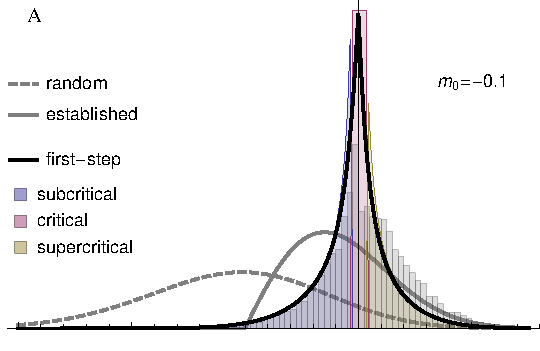
\includegraphics[width=\linewidth]{../IMAGES/firststep_smallm0_regimes.pdf}\\
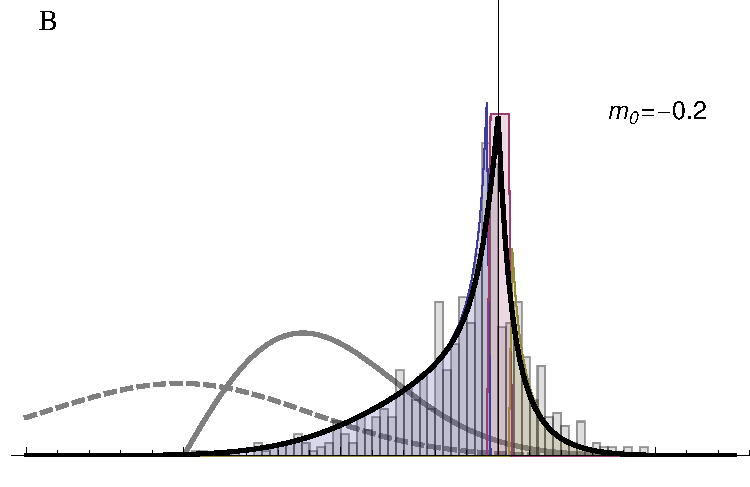
\includegraphics[width=\linewidth]{../IMAGES/firststep_medm0_regimes.pdf}\\
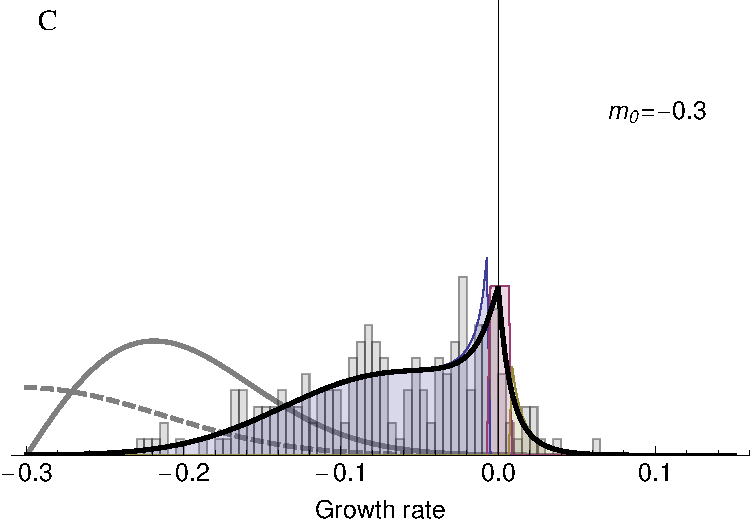
\includegraphics[width=\linewidth]{../IMAGES/firststep_largem0_regimes.pdf}\\
\caption{
The distribution of growth rates among first-step mutations that lead to 2-step rescue (black; Equation \ref{eq:hm}) for three different levels of initial maladaptation.
Shading represents our sufficiently subcritical approximation (blue; replacing $p(m,\Lambda_1(m))$ with $\Lambda_1(m)/|m|$ in the numerator of Equation \ref{eq:hm}), our sufficiently critical approximation (red; using $U f(0|m_0) \sqrt{2 \Lambda_1(0)}$ as the numerator in Equation \ref{eq:hm}), and our sufficiently supercritical approximation (yellow; replacing $p(m,\Lambda_1(m))$ with $\Lambda_1(m)/|m|$ in the numerator of Equation \ref{eq:hm}).
The histograms show the distribution of growth rates among first-step mutations in rescue genotypes with 2 mutations observed across (\textbf{A}, \textbf{B}) $10^5$ or (\textbf{C}) $10^6$ simulated replicates.
Note that the discrepancy in panel \textbf{A} is likely due to us sampling only the most common rescue genotype in each replicate.
See Figure \ref{fig:1and2stepDFE} for additional details.
}%
\label{fig:2stepDFE}
\end{figure}
%%%%%%%%%%%%%%%%%%%%%%%%%%%%%%%%%%%%%%%%%%%%%%%%%%%

%%%%%%%%%%%%%%%%%%%%%%%%%%%%%%%%%%%%%%%%%%%%%%%%%%%
%%%%%%%%%%%%%%%%%%%%%%%%%%%%%%%%%%%%%%%%%%%%%%%%%%%
\section{Discussion}
\label{sec:discussion}

Here we've explored the possibility of evolutionary rescue by multiple mutations on a simple fitness landscape. 
We find that rescue by multiple mutations can be the most likely path to persistence under high mutation rates or when the population is initially very maladapted.
Under these scenarios, intermediate genotypes that are declining less quickly provide a `springboard' from which rescue genotypes emerge.
In 2-step rescue these springboard single mutants come from one of three regimes: those that have growth rates near enough to zero (i.e., replacement) to, by chance, persist for unusually long periods of time and therefore reach unusually large subpopulation sizes and those with growth rates either too negative or too positive to do so.
The relative contribution of each regime shifts with initial maladaptation and mutation rate; rare mutations that can occasionally reach unusually large subpopulation sizes play a larger role as maladaptation declines and mutation increases.
In contrast, when initial maladaptation is very high most first-step mutations are themselves also very maladapted and thus restricted in the subpopulation sizes they reach.     
All three regimes help maintain the variance in the distribution of fitness effects among rescue genotypes as initial maladaptation increases; meanwhile, in 1-step rescue the variance declines due to ever more extreme sampling of the tail of the mutational distribution.

How often rescue arises as a result of multiple mutations is an open question. 
It is clear that more than one mutation can contribute to adaptation to near-lethal stress, but experiments are often designed to avoid extinction \citep[reviewed in][]{cowen2002evolution}, and therefore greatly expand the scope for multiple mutations to arise on a single genotype.
A few exceptions provide some insight.
For example, populations of \textit{Saccharomyces cervisae} that survived high concentrations of copper acquired multiple mutations \citep{Gerstein2015} -- in fact the authors argue for the `springboard effect' discussed above, where first step mutations prolong persistence and thereby allow further mutations to arise.
In \textit{Pseudomonas flourescens}, fluctuation tests with nalidixic acid showed that nearly a third of the most resistant surviving strains were double mutants \citep{Bataillon2011}, which were able to tolerate 10x higher drug concentrations than single mutants, suggesting 2-step rescue might dominate at high drug concentrations.
It is unclear if our prediction --  that rescue takes more mutational steps with greater initial maladaptation -- holds true. 
Verification will require more experiments that allow extinction and uncover the genetic basis of adaptation at different severities of environmental change (e.g., drug concentration).

In describing the genetic basis of adaptation in populations of constant size, \cite{Orr1998} showed that the mean phenotypic displacement towards the optimum scales roughly linearly with initial displacement.
Converting phenotype to fitness, this implies the mean fitness effect of fixed mutations, $s=m-m_0$, increases as $\sim \exp(-m_0)$ as initial Malthusian fitness, $m_0$, declines, which is roughly linear when $m_0$ is small.
Here we see that, under 1-step rescue, the mean fitness effect also increases roughly linearly as the initial growth rate declines (see horizontal blue lines in Figure \ref{fig:1and2stepDFE}).
However, the rate of this linear increase in fitness effect is much larger under rescue than in a population of constant size (compare blue and grey horizontal lines in Figure \ref{fig:1and2stepDFE}), where declines in wildtype fitness not only allow larger mutations to be beneficial but also require larger mutations for persistence.
Thus the race between extinction and adaptation during evolutionary rescue is expected to produce a genetic basis of adaptation with fewer mutations of larger effect.

While under 1-step rescue the fitness effect of the first mutation increases roughly linearly as wildtype fitness declines, below some wildtype fitness most rescue events will be 2-step (e.g., at $m_0 \approx -0.25$ in Figure \ref{fig:1vs2m0}).
At this junction the effect size of the first mutation will no longer increase as quickly (and potentially even decrease), as its expected fitness will itself begin to decline substantially with the fitness of the wildtype (Figures \ref{fig:2stepstyle} and \ref{fig:2stepDFE}).
Thus as rescue switches from dominantly $k$-step to dominantly $(k+1)$-step the genetic basis of adaptation becomes more diffuse, with each mutation having a smaller individual fitness effect as the contributing fitness effects spread over more loci.
In the limit of large $k$ (due to large initial maladaptation or high mutation rates), the genetic basis of adaptation should at some point converge to many loci with small effect, as would also be expected in a population of constant size.
Indeed, at very high mutation rates the rate of adaptation (the change in mean fitness) is the same under rescue as it is in populations of constant size \citep{anciaux2019population}, implying that the genetic basis of adaptation no longer depends on demography.
It is therefore at intermediate levels of initial maladaptation and low mutation rates, where rescue primarily occurs from a few large effect mutations, that the race between adaptation and persistence is predicted to have the largest effect on the genetic basis of adaptation.

%Fluctuation tests begin with a period of exponential population growth in a benign environment. 
%Exponential growth increases the probability that a new mutation establishes, relative to a population that is declining or constant in size \citep{Otto1997}, allowing many mutations reach relatively high frequencies. 
%These high frequencies then increase the probability of establishment that at least one copy of the mutation establishes in the selective environment. 
%Fluctuation tests therefore provide a means to assess the distribution of fitness effects among potential rescue mutants; it overweights those with small advantages in the selective environment, which are much less likely to establish in a declining population.
%Nevertheless, it is interesting to see that when the wildtype is unable to grow in the selective media the distribution of growth rates among potential rescue mutants can have both a mode and a minimum that are much larger than zero \citep{MacLean2009}.
%There are a number of possible explanations for this, including the fact that growth rates based on optical density above the minimal inhibitory concentration of a drug are difficult to interpret, potential sampling biases favouring larger effect mutations, and a finiteness in the mutational target.
%In contrast to fluctuation tests, exposing the ancestral population to strong selection -- without an initial prolonged period of exponential growth -- and isolating the survivors incorporates the probability of establishment and thus gives the distribution of fitness effects among realized rescue mutants. 
%Some such distributions qualitatively match our predictions \citep{Gerstein2012,Gerstein2015}, but others also include a minimum that is well above zero \citep{Lindsey2013}, again suggesting possible measurement error, sampling bias, or finite mutational targets.
%Interestingly, this latter example found that the distribution of growth rates varied little with the rate at which drug concentration increased, which might indicate support for our prediction that the distribution of growth rates among rescue mutants is expected to change relatively little with initial maladaptation (Figure \ref{fig:1and2stepDFE}).
%Our theory predicts that the distribution of growth rates among rescue genotypes, sampled across many replicates, will have a minimum very near zero and substantially positive mode (as opposed to, say, an exponential distribution). 
Fluctuation tests \citep{luria1943mutations} provide a means to isolate rescue genotypes, whose growth rates can then be measured under the selective conditions.
Consistent with our theory (Figure \ref{fig:1and2stepDFE}), the resulting growth rate distributions in both bacteria and yeast often find modes that are substantially greater than zero \citep[as opposed to, say, an exponential distribution;][]{Kassen2006,MacLean2009,Gerstein2012,Lindsey2013,Gerstein2015}.
A number of these conform even more closely to our expected shape \citep{Kassen2006,Gerstein2015} while the others appear to be substantially more clumped around the mode, perhaps due to a very restricted number of possible rescue mutations in any one circumstance, the size of the experiment, or the way in which growth rates are measured.
Further, these experiments are designed to begin with substantial standing genetic variation (at least across replicates), which should increase the contributions of mutations with small growth rates \citep{orr2001haldane}, although these could be outcompeted by mutations with higher growth rates and/or be undersampled.
The role of standing genetic variance becomes particularly important when we consider rescue by multiple steps, as the ability of the intermediate genotypes to persist long enough to accumulate further mutations will differ strongly between environments.
Finally, \cite{Gerstein2015} not only provides the distribution of growth rates among rescue genotypes, but also the growth rates of individual mutations that compose multi-step rescue genotypes.
In two of three cases they see that most component mutations have growth rates near that of the multi-mutation genotype while in the other case there appears to be multiple mutations that provide intermediate benefits, consistent with their hypothesis of multi-step rescue.
These growth rates were measured in a less stressful environment than the original selective environment, which unfortunately makes it impossible to tell if these individual mutations had positive or negative growth rates (i.e., were subcritical or supercritical) during rescue.

Pinpointing the mutations responsible for adaptation is hampered by genetic hitchhiking, as beneficial alleles elevate the frequency of linked neutral and mildly deleterious alleles \citep{barton2000genetic}.
The problem is particularly severe under strong selection and low recombination, and therefore reaches an extreme in the case of evolutionary rescue in asexuals, especially if many neutral and deleterious mutations are segregating at the time of environmental change.
To circumvent this, mutations that have risen to high frequency in multiple replicates are often introduced in a wildtype background, in isolation and sometimes also in combination with a small number of other common high-frequency mutations, and grown under the selective conditions \citep[e.g.,][]{jochumsen2016evolution,ono2017widespread}.
As we have demonstrated above, however, under multi-step rescue there may be no one mutation that individually confers growth in the selective conditions.
Thus, a mutation driving rescue may go undetected or be mistaken as a hitchhiker if the appropriate multiple-mutation genotypes are not tested. 
Unfortunately reverse engineering all combinations of mutations quickly becomes unwieldy as the number of mutations grows, and thus this approach will not be practical under severe initial maladaptation and high mutation rates, where we predict rescue to occur by many mutations.
Interestingly, our simulations show that the population dynamics themselves may help differentiate how many mutations contribute to rescue (e.g., V- vs.\ U-shaped log-trajectories; Figures \ref{fig:Vshape} and \ref{fig:Ushape}), and fitting models of $k$-step rescue could produce estimates for the growth rates of the $k$ genotypes.

Environmental change often selects for mutator alleles, which elevate the rate at which beneficial alleles arise and subsequently increase in frequency with them \citep{tenaillon2001second}.
When beneficial alleles are required for persistence, as in evolutionary rescue, mutator alleles can reach very high frequencies or rapidly fix \citep[e.g.,][]{mao1997proliferation}.
Consistent with this, mutator alleles are often associated with antibiotic resistance in clinical isolates \citep[see examples in][]{Bell2017}.
Further, the more beneficial mutations available the larger the advantage of a mutator allele; for a mutator that increases the mutation rate $m$-fold, its relative contribution to the production of $n$ beneficial mutations scales as $m^n$ \citep{tenaillon1999mutators}.
Thus multi-step rescue can impose much stronger selection for mutator alleles than 1-step rescue.
There are a number of examples where lineages with higher mutation rates acquired multiple mutations and persisted at higher doses of antibiotics \citep{couce2015bypass,san2017multicopy}.
The number of mutations required for persistence is, however, often unknown, making it difficult to compare situations where rescue requires different numbers of mutations.
Experiments with a combination of drugs may provide a glimpse; for instance, \textit{Escherichia coli} populations only evolved resistance to a combination of two drugs (presumably through the well-known mutations specific to each drug) when mutators were present, despite the fact that mutators were not required for resistance to either drug in isolation \citep{gifford2019mutators}. 
In cases where we have less information on the genetic basis of resistance, our model suggests that mutators will be more advantageous when initial maladaptation is severe (e.g., higher drug concentrations or a larger number of drugs), as rescue will then be dominated by genetic paths with more mutational steps.

Here we have investigated the genetic basis of evolutionary rescue in an asexual population that is initially genetically uniform. 
Extending this work to allow for recombination and standing genetic variation at the time of environmental change will likely be interesting. 
The effect of standing genetic variation on the probability of 1-step rescue is relatively straight-forward to incorporate, depending only on the expected number of rescue mutations initially present and their mean establishment probability \citep{Martin2013}. 
In the case of mutation-selection balance, the probability of 1-step rescue from standing genetic variance in Fisher's geometric model was given by \cite{Anciaux2018}, whose equations 3 and 5 immediately give the distribution of fitness effects among those that rescue.
Allowing these standing genetic variants to be springboards to multi-step rescue will help clarify the role of standing genetic variation on the genetic basis of rescue more generally.
Recombination can help combine such springboard mutations into rescue genotypes but will also break these combinations apart, as demonstrated in a 2-locus 2-allele model of rescue \citep{Uecker2016}.
How recombination affects the genetic basis of evolutionary rescue when more loci can potentially contribute remains to be seen.

%%%%%%%%%%%%%%%%%%%%%%%%%%%%%%%%%%%%%%%%%%%%%%%%%%%
%%%%%%%%%%%%%%%%%%%%%%%%%%%%%%%%%%%%%%%%%%%%%%%%%%%
\section{Acknowledgements}

We would like to thank the Otto and Doebeli labs for helpful feedback at various stages, Oph\'{e}lie Ronce and Thomas Lenormand for their hospitality and valuable input at the beginning of this project, and Mike Whitlock, Amy Angert, and Luis-Miguel Chevin for constructive criticism on previous versions of the manuscript.
Funding provided by the National Science and Engineering Research Council (CGS-D 6564 to M.M.O., RGPIN-2016-03711 to S.P.O.), the University of British Columbia, Banting, and the University of California - Davis (fellowships to M.M.O.), the National Institute of General Medical Sciences of the National Institutes of Health (NIH R01 GM108779 to Graham Coop), the Agence Nationale de la Recherche (ANR-18-CE45-0019 "RESISTE" to G.M.), and the Centre M\'{e}diterran\'{e}en Environment et Biodiversit\'{e} ("BACTPHI" to G.M.).

%%%%%%%%%%%%%%%%%%%%%%%%%%%%%%%%%%%%%%%%%%%%%%%%%%%
%%%%%%%%%%%%%%%%%%%%%%%%%%%%%%%%%%%%%%%%%%%%%%%%%%%
\bibliography{extracted}

%%%%%%%%%%%%%%%%%%%%%%%%%%%%%%%%%%%%%%%%%%%%%%%%%%%
%%%%%%%%%%%%%%%%%%%%%%%%%%%%%%%%%%%%%%%%%%%%%%%%%%%
\section{Appendix}
\label{sec:appendix}
%\setcounter{equation}{0}
%\renewcommand{\theequation}{A\arabic{equation}}

\subsection{Approximating the probability of 1-step rescue}
\label{subsec:1stepApproximations}

The probability of 1-step rescue in this model has been derived by \cite{Anciaux2018}.
As replicated in File S1 and given by their equation 7, when $\rho_{max} = m_{max}/\lambda$ is large a closed-form approximation is

\begin{equation}\label{eq:p1closed}
\Lambda_1(m_0) \approx \tilde{\Lambda}_1(m_0) \equiv  -m_0 U \frac{(1-\psi_0/2)^{(1-n)/2}}{1-\psi_0/4} g(\alpha),
\end{equation}

\noindent where $\psi_0 = 2(1-\sqrt{1-m_0/m_{max}})$, $g(\alpha) = \exp(-\alpha)/\sqrt{\pi \alpha} - \mathrm{erfc}(\sqrt{\alpha})$, and $\alpha=\rho_{max} \psi_0^2/4$, with $\mathrm{erfc}(.)$ the complimentary error function.
When the wildtype declines slowly $m_0$ and thus $\psi_0$ is small and $\Lambda_1(m_0)\approx U g(\alpha)$.
In the limit $m_0\rightarrow0$, Equation \ref{eq:p1closed} becomes

\begin{equation}\label{eq:Lambda0}
\tilde{\Lambda}_1(0) \equiv \lim_{m_0\rightarrow0} \tilde{\Lambda}_1(m_0) = 2 U \sqrt{m_{max}\lambda/\pi}.
\end{equation} 

\subsection{Mutant lineage dynamics}
\label{subsec:mutants}

Here we follow the lead of \cite{Weissman2010} and \cite{Uecker2016} in approximating our discrete-time process with a continuous-time branching process \citep[see chapter 6 in][]{Allen2010}. 
Consider a birth-death process, where individuals give birth at rate $b$ and die at rate $d$. 
One can then obtain the probability generating function for the number of individuals at a given time, $n(t)$, given the initial number, $n(0)$.
We are primarily interested in new mutant lineages, $n(0)=1$.
The generating function then allows us to calculate the probability that a lineage persists at least until time $t$ and the distribution of $n(t)$ given it does so (see below).

To convert between birth and death rates and our compound Malthusian parameter we follow \cite{Uecker2016} in equally distributing the growth rate $m$ between birth and death, $b = (1+m)/2$ and $d=(1-m)/2$, such that $m=b-d$ and the continuous-time process exhibits the same amount of drift as the discrete time process \citep[and matches discrete-time simulations well;][]{Uecker2014}.
We can now report the necessary results in terms of $m$ (assuming $|m|<1$).

Denoting the extinction time as $T$, the probability a mutant with growth rate $m$ persists until time $t$ is approximately (see File S1 for derivation)

\begin{equation}\label{eq:pT}
P( T > t ) \approx 
\begin{cases}
	2 / t & t << |1/m| \\
	-2 m \exp(m t) & t >> -1/m > 0
\end{cases}
\end{equation}

\noindent As pointed out in \cite{Weissman2010} (whose equation A2 differs from Equation \ref{eq:pT} by a factor of 2 because they have $b+d=2$), the distribution of persistence times has a long tail (like $1/t$) until being cut off (declining exponentially) at $t=-1/m$.

Given a lineage persists until $t$, the distribution of $n(t)$ is roughly (see File S1 for derivation)

\begin{equation}\label{eq:pnt}
P( n(t) = n | n(t) > 0 ) \approx 
\begin{cases}
	2 (1/t) (1 + 2/t)^{-n} & t << |1/m| \\
	-2 m (1 + m)^{n-1} & t >> -1/m > 0
\end{cases}
\end{equation}

\noindent As pointed out in \cite{Weissman2010} (whose equation A3 only differs from Equation \ref{eq:pnt} by constants), the distribution of $n(t)$ is approximately geometric for small or large $t$, implying $n(t)$ is very unlikely to be greater than the minimum of $t$ and $-1/m$.

%%%%%%%%%%%%%%%%%%%%%%%%%%%%%%%%%%%%%%%%%%%%%%%%%%%
%\section{Supplementary figures}
\setcounter{figure}{0}
\renewcommand{\thefigure}{S\arabic{figure}}
\setcounter{table}{0}
\renewcommand{\thetable}{S\arabic{table}}

%%%%%%%%%%%%%%%%%%%%%%%%%%%%%%%%%%%%%%%%%%%%%%%%%%%
\begin{figure}[htbp]
\centering
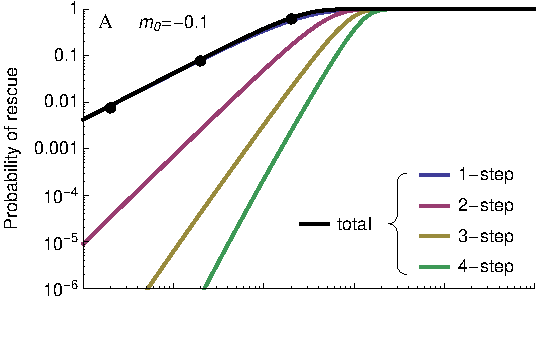
\includegraphics[width=\linewidth]{../IMAGES/4step_lowm0.pdf}\\
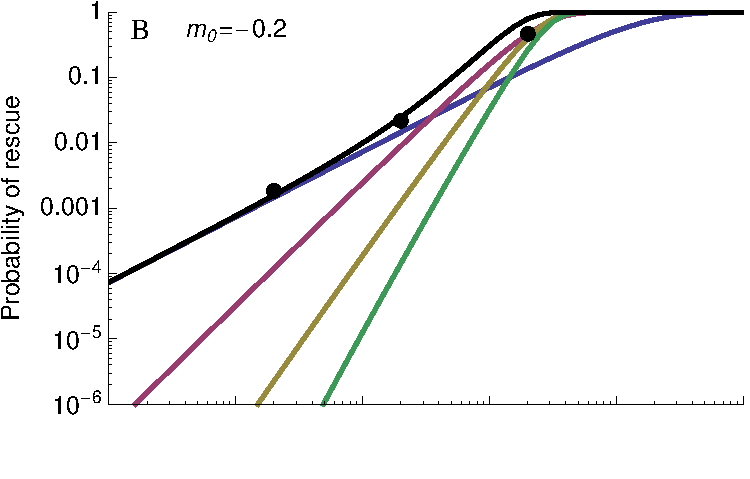
\includegraphics[width=\linewidth]{../IMAGES/4step_medm0.pdf}\\
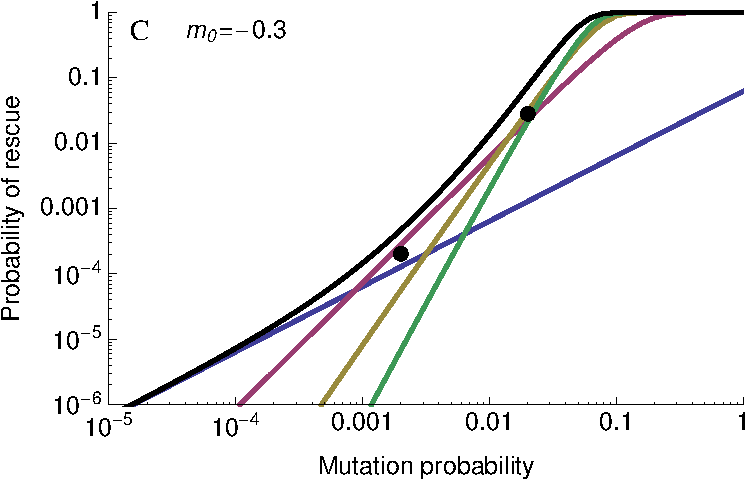
\includegraphics[width=\linewidth]{../IMAGES/4step_highm0.pdf}\\
\caption{
The probability of rescue as a function of mutation rate for three different levels of initial maladaptation.
See Figure \ref{fig:1vs2m0} for details.
Other parameters: $n=4$, $\lambda=0.005$, $m_{max}=0.5$, $N_0=10^4$.
}%
\label{fig:1vs2U}
\end{figure}
%%%%%%%%%%%%%%%%%%%%%%%%%%%%%%%%%%%%%%%%%%%%%%%%%%%

%%%%%%%%%%%%%%%%%%%%%%%%%%%%%%%%%%%%%%%%%%%%%%%%%%%
\begin{figure}[htbp]
\centering
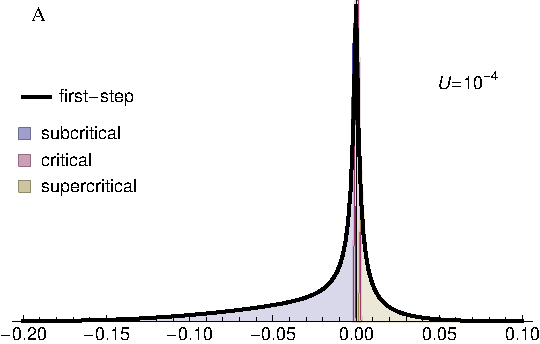
\includegraphics[width=\linewidth]{../IMAGES/firststep_smallU.pdf}\\
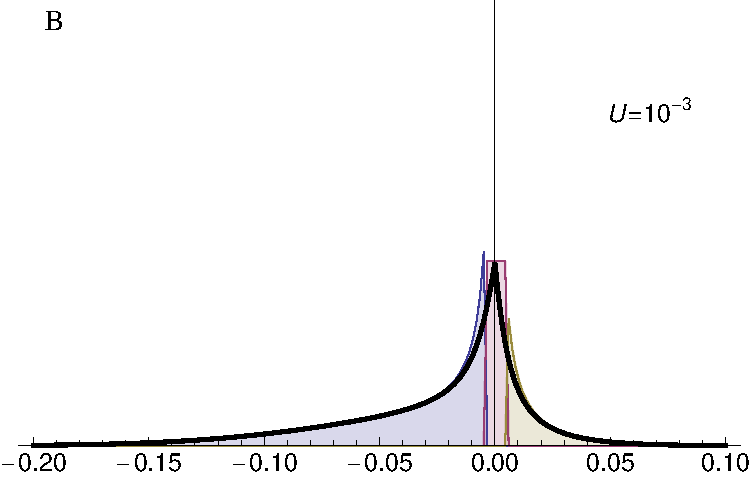
\includegraphics[width=\linewidth]{../IMAGES/firststep_medU.pdf}\\
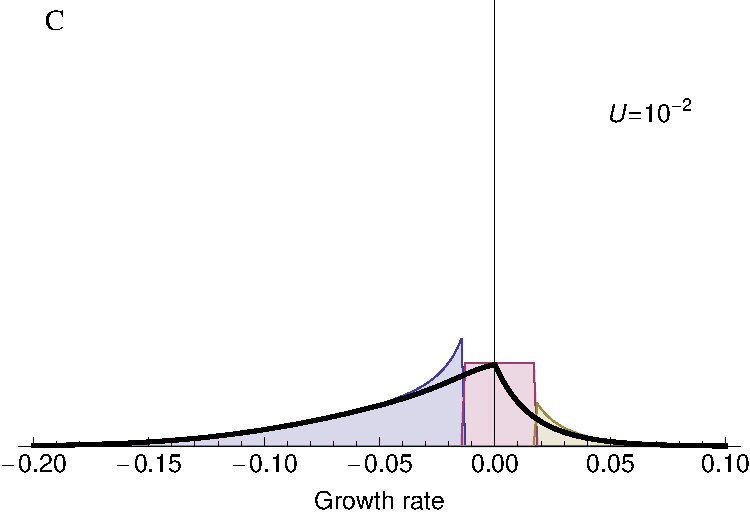
\includegraphics[width=\linewidth]{../IMAGES/firststep_largeU.pdf}
\caption{
The distribution of first-step mutant growth rates given 2-step rescue under three mutation rates. 
See Figure \ref{fig:2stepDFE} for details.
Parameters: $n=4$, $\lambda=0.005$, $m_{max}=0.5$, $m_0=-0.2$.
}%
\label{fig:firststepDFE_mutation}
\end{figure}
%%%%%%%%%%%%%%%%%%%%%%%%%%%%%%%%%%%%%%%%%%%%%%%%%%%

\end{document}